%%%%%%%%%%%%%%%%%%%%%%%%%%%%%%%%%%%%%%%%%%%%%%%%%%%%%%%%%%%%%%%%%%%%%%%%%%%%%%%
% Author:  Pablo Alvarado
%
% School of Electronic Engineering
% Costa Rica Institute of Technology
%
% Licentiate Thesis
% 
% Phone:   +506 550 2106
% Fax:     +506 591 6629
% email:   palvarado@ietec.org
%
% $Id: main.tex 1513 2010-08-15 01:25:24Z palvarado $
%
% Modified by Yeiner Arias for use in
% the School of Mechatronics Engineering
%%%%%%%%%%%%%%%%%%%%%%%%%%%%%%%%%%%%%%%%%%%%%%%%%%%%%%%%%%%%%%%%%%%%%%%%%%%%%%%

\documentclass[12pt,twoside,letterpaper]{book}

\usepackage[utf8]{inputenc}
\usepackage{ifthen}                     % provide if-then-else operators

% --------------------------------------------------------------------------
% Global variables required in document formatting
% --------------------------------------------------------------------------

\newboolean{bookmode}                  
\setboolean{bookmode}{true}

\newboolean{draftmode}                  
\setboolean{draftmode}{false}

% GENERAL AUTHOR, TITLE AND KEYWORDS
\newcommand{\scriptAuthor}{First Name Last Name}
\newcommand{\scriptTitle}{An MBSE-Based Framework for the Design and Analysis of Nanosatellite Electrical Power Systems} 
\newcommand{\scriptKeywords}{keywords, ...}

\newcommand{\boxeditorial}{%
}

\newcommand{\pdfAuthor}{\scriptAuthor}
\newcommand{\pdfTitle}{\scriptTitle} 
\newcommand{\pdfKeywords}{\scriptKeywords}

% --------------------------------------------------------------------------

% include all packages and define all required general macros
%%%%%%%%%%%%%%%%%%%%%%%%%%%%%%%%%%%%%%%%%%%%%%%%%%%%%%%%%%%%%%%%%%%%%%%%%%%%%%%
% Author:  Pablo Alvarado
%
% Escuela de Electrónica
% Instituto Tecnológico de Costa Rica
%
% Phone:   +506 550 2106
% Fax:     +506 591 6629
% email:   palvarado@ietec.org
%
% $Id: macros.tex 1497 2010-08-09 17:04:26Z palvarado $
%

%Versión modificada por Yeiner Arias para uso en
%la Escuela de Imgeniería Mecatrónica
%%%%%%%%%%%%%%%%%%%%%%%%%%%%%%%%%%%%%%%%%%%%%%%%%%%%%%%%%%%%%%%%%%%%%%%%%%%%%%%

% Configuration of the exercises package, which is used to collect all
% problems and answers in the document.
\usepackage[exercisedelayed,answerdelayed,lastexercise]{exercise}
\renewcounter{Exercise}[chapter]
\renewcommand{\ExerciseName}{Problema}
\renewcommand{\theExercise}{\thechapter.\arabic{Exercise}}
\newcommand{\ExerciseLabel}{Exercise.\theExercise}
\renewcommand{\ExerciseHeader}%
{\textbf{\ExerciseName\ \theExercise.\ \ExerciseHeaderTitle\ }}
\renewcommand{\AnswerHeader}%
{\textbf{\ExerciseName\ \theExercise.\ }}


\usepackage{ifpdf}

% Command to change between draft or release mode:
\newcommand{\ifdraft}[2]{\ifthenelse{\boolean{draftmode}}{#1}{#2}}
% Command to change between draft or release mode:
\newcommand{\ifbook}[2]{\ifthenelse{\boolean{bookmode}}{#1}{#2}}

% include all required packages here
\usepackage[spanish,english]{babel}     % supports english, but default is 
                                        % spanish...
\newcommand*{\SelectSpanish}{%          % well, the last line indeed selects
  \hyphenrules{spanish}%                % english over spanish, but with this
  \languageshorthands{spanish}%         % command we turn it around.
  \captionsspanish                      % The reason: hyperref has some
  \datespanish                          % problems with the spanish babel,
}                                       % so we use some trick here so that it
\AtBeginDocument{\SelectSpanish}        % thinks it is english.

\usepackage{makeidx}                    % to create index file

\ifdraft{%
  %\usepackage[refpage]{nomencl}        % Use to easily administrate the list
 \usepackage{nomencl}                   % of symbols
}{%
 \usepackage{nomencl}
}
%\usepackage{times}                     % replace latex pk fonts with ps type I
                                        % don't forget to use dvips -D600 -Pcmz
                                        % to ensure Type I fonts!
\usepackage{amsmath}
\usepackage{amssymb,amstext}            % AMS-math and symbols package
\usepackage[numbers,sort&compress]{natbib} % citation commands and formatting
\usepackage{mathrsfs}                   % Calygraphic fonts for transforms
\usepackage{array}                      % extensions to tabular environment
\usepackage{longtable}                  % supports extraordinary long tables
\usepackage{tabularx}                   % supports tables with fixed width
\usepackage{afterpage}                  % put something only after the page
\usepackage{multirow}                   % supports multiple row grouping in 
                                        % tables
\usepackage{multicol}                   % multiple columns environments
\usepackage{paralist}                   % a few enumeration settings

\usepackage{bigstrut}

\usepackage[table]{xcolor}

\usepackage{multirow}

\usepackage[hang,%
            small,%
            bf]{caption}                % nicer figure captions
%\usepackage{sty/ftcap}                 % switch \abovecaptionskip and
%                                       % \belowcaptionskip for tables, in 
%                                       % order to avoid the caption to be
%                                       % too near to the table itself
% locally added packages
\usepackage{float}                      % really place figures "here" (H)
\usepackage{booktabs}                   % book type tabulars
% Presentation-only additions. The existing report macros remain unchanged.
% enumitem defines a separate list type. No global itemize/enumerate changes.
\usepackage{enumitem}
\usepackage{needspace}
\usepackage{pdflscape} % Full-page, reader-rotated logical exchange panels.
\newlist{causes}{itemize}{5}
\setlist[causes]{label=\textbullet,leftmargin=1.15em,labelsep=.35em,
  itemsep=.20\baselineskip,parsep=0pt,topsep=.20\baselineskip,
  partopsep=0pt,before={\raggedright\clubpenalty=10000\widowpenalty=10000}}
% Five child levels are available. With the root paragraph this supports six
% total causal levels. The baseline currently needs four child levels.
\makeatletter
\newcommand{\ConcernAnchor}[1]{%
  \phantomsection
  \begingroup\def\@currentlabel{#1}\label{concern:#1}\endgroup}
\makeatother
\newcommand{\ConcernId}[1]{\mbox{\textsf{#1}}}
\newcommand{\ConcernRef}[1]{\hyperref[concern:#1]{\ConcernId{#1}}}
\newcommand{\ConcernRole}[1]{\par\Needspace{7\baselineskip}\subsubsection*{#1}}
\newcommand{\ConcernRoot}[2]{%
  \par\addvspace{.7\baselineskip}\Needspace{4\baselineskip}%
  \begingroup\raggedright
  \ConcernAnchor{#1}\noindent\textbf{\ConcernId{#1}}\quad #2\par\endgroup}
\newcommand{\ConcernCause}[2]{%
  \item\leavevmode\ConcernAnchor{#1}{\small\textbf{\ConcernId{#1}}}\quad #2}
\newcommand{\ConcernAliasLink}[1]{\space(see \ConcernRef{#1})}
\newcommand{\ConcernSummary}[2]{%
  \par\addvspace{.7\baselineskip}\Needspace{4\baselineskip}%
  \begingroup\raggedright
  \ConcernAnchor{#1}\noindent\textbf{\ConcernId{#1}}\quad #2\par\endgroup}

% Table recipes use exactly the available line width. Padding is included.
\newlength{\ReportTableBodyWidth}
\newcommand{\ReportTableSetup}[1]{%
  \small
  \setlength{\tabcolsep}{4pt}%
  \setlength{\ReportTableBodyWidth}{\dimexpr\linewidth-#1\tabcolsep\relax}%
  \renewcommand{\arraystretch}{1.15}}
\newcolumntype{P}[1]{>{\raggedright\arraybackslash}p{#1}}
            % isolated concern and trace formatting

% the own style with options depending on the draft mode
\ifdraft{%
\usepackage[todo]{sty/tecStyle}         % some command definitions
                                        % options [todo] todo-index
}{%
\usepackage{sty/tecStyle}               % some command definitions
                                        % options [todo] todo-index
}

%% fix the title for examples
\renewcommand{\examplelistname}{Índice de ejemplos}
\renewcommand{\examplename}{Ejemplo}


\usepackage{url}                        % allows linebreaks at certain
                                        % characters or combinations of 
                                        % characters for URLs

%\usepackage[nottoc]{tocbibind}          % Fix the hyperrefs to TOC,TOF, etc.
                                        % and ensure that they appear all in 
                                        % the Table of Contents

\definecolor{dkred}{rgb}{0.5,0,0}       %   dark red
\definecolor{dkgreen}{rgb}{0,0.3,0}     %   dark green
\definecolor{dkblue}{rgb}{0,0.0,0.5}    %   dark blue
\definecolor{dkgray}{gray}{0.4}         %   dark gray
\definecolor{dkmagenta}{rgb}{0.3,0.0,0.3} % dark magenta
\definecolor{ltyellow}{rgb}{1.0,1.0,0.7}  % light yellow

\newcommand{\bG}[1]{\textcolor{dkgreen}{\textbf{#1}}}
\newcommand{\bR}[1]{\textcolor{dkred}{\textbf{#1}}}
\newcommand{\bB}[1]{\textcolor{dkblue}{\textbf{#1}}}
\newcommand{\bM}[1]{\textcolor{dkmagenta}{\textbf{#1}}}
\newcommand{\bY}[1]{\textcolor{dkyellow}{\textbf{#1}}}
\newcommand{\bC}[1]{\textcolor{dkcyan}{\textbf{#1}}}

% For pdflatex
% - The hyperref package should always be loaded last, since it has to
%   overwrite some of the commands.
% - The package subfigure caused that the pagebackrefs and index refs were set
%   incorrectly.

\ifpdf
%
% final / draft document options
\usepackage[pdftex,final]{graphicx}     % for inserting pdf-graphics.
                                        % options final / draft
\ifdraft{%

\usepackage[pdftex,%
            pdftitle={\pdfTitle},%
            pdfauthor={\pdfAuthor},%
            pdfsubject={Notas de Clase},%
            pdfkeywords={\pdfKeywords},%
            naturalnames=true,
            linktocpage,
            hyperindex,
            colorlinks,
            urlcolor=dkred,          %\href to external url
            filecolor=dkmagenta,     %\href to local file
            linkcolor=dkred,         %\ref and \pageref
            citecolor=dkgreen,       %\cite
            pagebackref,
            plainpages=false,
            pdfpagelabels,
            pdfpagemode=UseOutlines, % means use bookmarks (None,UseOutlines)
            % bookmarksopen=false,   % would show the whole hierarchy if true
            bookmarksnumbered=true,
            pdfpagelayout=OneColumn, % SinglePage,OneColumn,TwoColumnLeft,...
            pdfview=FitH, % FitB,FitBH,FitBV,Fit,FitH,FitV
            pdfstartview=FitH, % FitB,FitBH,FitBV,Fit,FitH,FitV
            ]{hyperref}
}{%
\usepackage[pdftex,%
            pdftitle={\pdfTitle},%
            pdfauthor={\pdfAuthor},%
            pdfsubject={Notas de clase},%
            pdfkeywords={\pdfKeywords},%
            naturalnames=true,
            linktocpage,hyperindex,
            colorlinks,
            urlcolor=dkred,          %\href to external url
            filecolor=dkmagenta,     %\href to local file
            linkcolor=dkred,         %\ref and \pageref
            citecolor=dkgreen,       %\cite
            % pagebackref,           % only in draft modus should this be on.
            plainpages=false,
            pdfpagelabels,
            pdfpagemode=UseOutlines, % means use bookmarks (None,UseOutlines)
            % bookmarksopen=false,   % open the whole hierarchy if true!
            bookmarksnumbered=true,
            pdfpagelayout=OneColumn, % SinglePage,OneColumn,TwoColumnLeft,...
            pdfview=FitH, % FitB,FitBH,FitBV,Fit,FitH,FitV
            pdfstartview=FitH, % FitB,FitBH,FitBV,Fit,FitH,FitV
            ]{hyperref}
}

%
% Ensure that the links of the images point to the top of the images and not
% to the caption
%
\usepackage[figure]{hypcap}
\usepackage{algorithm}
\usepackage{algpseudocode}

% %
% % Ensure that pdfLaTeX do the same spacing as LaTeX
% %
\pdfadjustspacing=1 
% %
\else   % i.e. if not pdf

\usepackage[active]{srcltx}             % insert links into the dvi to jump
\usepackage[dvips,final]{graphicx}      % for inserting eps-graphics.
                                        % options final / draft
                                        % into the sources directly.
\ifdraft{%
\usepackage[ps2pdf,%
            pdftitle={\pdfTitle}%
            pdfauthor={\pdfAuthor},%
            pdfsubject={Notas de clase},%
            pdfkeywords={\pdfKeywords},%
            % plainpages=false,
            linktocpage,
            hyperindex,
            pagebackref,
            % pdfpagelabels,
            pdfpagemode=UseOutlines,
            pdfstartview=FitH]{hyperref}
}{%
\usepackage[ps2pdf,%
            pdftitle={\pdfTitle}%
            pdfauthor={\pdfAuthor},%
            pdfsubject={Notas de clase},%
            pdfkeywords={\pdfKeywords},%
            % plainpages=false,
            linktocpage,
            hyperindex,
            % pagebackref,
            % pdfpagelabels,
            pdfpagemode=UseOutlines,
            pdfstartview=FitH]{hyperref}
}

%\usepackage[ps2pdf]{hyperref}

\fi  % end of if pdf or not

\usepackage{tikz}
\usetikzlibrary{arrows.meta,shapes.geometric,babel}
\usepackage{rotating}                   % allow block rotation


%%%%%%%%%%%%%%%%%%%%%%%%%%%%%%%%%%%%%%%%%%%%%%%%%%%%%%%%%%%%%%%%%%%%%%%%%%%%%%%

%\sloppy

%
% Some own font definitions
%
\DeclareMathAlphabet{\mathpzc}{OT1}{pzc}{m}{it}
\DeclareMathAlphabet{\mathpss}{OT1}{cmss}{m}{sl}

%
% page layout
%

\usepackage{vmargin}
\setpapersize{USletter}

\ifbook{%
% left,top,right,bottom,headheight,headsep,footheight,footsep
%
% For the book legal-paper printing (two pages per legal paper)
\setmarginsrb{31mm}{8mm}{20mm}{7mm}{15pt}{15pt}{7mm}{9mm}
%\setmarginsrb{33mm}{8mm}{23mm}{7mm}{15pt}{15pt}{7mm}{12mm}
}{%
% For letter-paper printing
\setmarginsrb{33mm}{8mm}{23mm}{7mm}{15pt}{15pt}{7mm}{12mm}
}
%\setlength{\headheight}{15pt}         % fancy headers wanted this

%
% Fraction of Float Object / Text
%

\renewcommand{\topfraction}{0.95}       % how much of top of page should be 
                                        % allowed to be float object?
\renewcommand{\bottomfraction}{0.95}    % how much of bottom of page should be
                                        % allowed to be float object?
\renewcommand{\textfraction}{0.05}      % how much of page must be text?

\usepackage{fancyhdr}                   % fancy page headers

\usepackage{lastpage}

%
% header and footer layout (needs package fancyhdr)
%
\newcommand{\copyrightfooter}{\tiny{\copyright 2005-2010 --- P.~Alvarado %
    \qquad Uso exclusivo ITCR}}
%
\newcommand{\draftfoot}%
  {\ifdraft{\textcolor{dkblue}{\tiny\textsl{Borrador: \today}}{}}
           {}
}

\pagestyle{fancy}
\renewcommand{\chaptermark}[1]{\markboth{{\small
    \thechapter\hspace*{1mm}#1}}{}}
\renewcommand{\sectionmark}[1]{\markright{{\small
    \thesection\hspace*{1mm}#1}}{}}
\lhead[{\small\textbf\thepage}]{\fancyplain{}%
        {{\slshape \small\nouppercase{\leftmark}}}}
\chead[]{}
\rhead[\fancyplain{}%
        {{\slshape \small\nouppercase{\rightmark}}}]{{\small\textbf\thepage}}
\lfoot[]{\draftfoot}
\ifbook{%
  \cfoot[]{}
}{
  \cfoot[\copyrightfooter]{\copyrightfooter}
}
\rfoot[\draftfoot]{}
\renewcommand{\headrulewidth}{0.5pt}
\renewcommand{\footrulewidth}{0pt}


% Activa el color de las filas de las tablas
%	#1	Posición inicial del inicio de colores
\newcommand{\enabletablerowcolor}[1][]{%
	\ifx\hfuzz#1\hfuzz%
		\settablerowcolors{2}%
	\else%
		\settablerowcolors{#1}%
	\fi%
}

% Desactiva el color de las filas de las tablas
\newcommand{\disabletablerowcolor}{\rowcolors{2}{}{}}

%
% Caption style for tables
% Requires the packages caption2 and ftcap
% (caption2 required this, but is obsolete now:)
%
%\newcaptionstyle{tablecaptionstyle}{%
%  \renewcommand\captionlabelfont{\normalsize\bf}
%  \renewcommand\captionfont{\normalsize}
%  \usecaptionstyle{hang}%
%}

% For caption v3:

\newcommand{\tablecaption}[2][foo]{%
  \ifthenelse{\equal{#1}{foo}}{%
    %\captionstyle{tablecaptionstyle}%
    \caption{#2}%
  }
  {%
    %\captionstyle{tablecaptionstyle}%
    \caption[#1]{#2}%
  }
}
\addto\extrasspanish{\renewcommand{\tablename}{Tabla}}
\addto\extrasspanish{\renewcommand{\listtablename}{\'Indice de tablas}}

%
% paragraph layout
%
\renewcommand{\baselinestretch}{1.1}    % line spacing
\parindent0em                           % indentation width of first line
\parskip1.3ex                           % space between paragraphs

%
% document consists of
% chapter - section - subsection - subsubsection - paragraph - subparagraph
%
\setcounter{secnumdepth}{2}             % depth of section numbering
\setcounter{tocdepth}{2}                % depth of table of contents

%
% prepares index from entries like \index{word} or \index{group!word}.
% don't forget to call "makeindex filename" for final index generation.
%
\makeindex                            %% for package makeidx.sty
%\newindex{default}{idx}{ind}{Index}  %% for package index.sty

\newcommand{\octave}{GNU/Octave}


%
% prepares notation or nomenclature 
%
%\makeglossary
\makenomenclature

%%% Local Variables: 
%%% mode: latex
%%% TeX-master: "main"
%%% End: 

\allowdisplaybreaks[3]

% --------------------------------------------------------------------------
\begin{document}
  \graphicspath{{./}{./fig/}}

  \pagenumbering{alph}
  \renewcommand{\tablename}{Table}
  \renewcommand{\listtablename}{List of Tables}
  \renewcommand{\examplesolution}{Solution}
  \pagestyle{empty}

  %% ---------------------------------------------------------------------------
%% titlepage.tex
%%
%% Title page
%%
%% $Id: titlepage.tex 1452 2010-07-07 00:55:16Z palvarado $
%% ---------------------------------------------------------------------------

\thispagestyle{empty} 

\begin{center}

Costa Rica Institute of Technology

\par\vspace{1ex}

School of Mechatronics Engineering

\par\vspace{20mm}


\includegraphics[width=70mm]{TEC}

\par\vspace*{\fill}

{\large\bf{\scriptTitle}}

\par\vspace*{\fill}

Graduation Project Report submitted for the degree of

Licentiate in Mechatronics Engineering



\par\vspace{20mm}

\scriptAuthor

\vspace*{\fill}

\ifdraft{%
{Draft of \today}
}{
Cartago, \today}
\end{center}
\newpage 
\cleardoublepage 


%%% Local Variables: 
%%% mode: latex
%%% TeX-master: "main"
%%% End: 

  \thispagestyle{empty}

\rule{10mm}{0pt}

\vfill

I declare that I completed this Graduation Project entirely myself, using
and applying relevant literature and contributing my own knowledge.

I have acknowledged all sources through the corresponding bibliographic
citations. I take full responsibility for this graduation project and the
content of its final report.



\vspace*{8mm}

\begin{flushright}
  \scriptAuthor\par
  Cartago, \today\par
  National ID: X-XXXX-XXXX
\end{flushright}

\cleardoublepage

%%% Local Variables: 
%%% mode: latex
%%% TeX-master: "main"
%%% End: 

  \chapter*{Abstract}
\thispagestyle{empty}

For the ASCEND research group at the École de technologie supérieure, evidence fragmentation during the early lifecycle phases of nanosatellite electrical power systems hinders the traceability between needs and requirements, architecture decisions, and the analytical evidence that supports them. Furthermore, it hinfers the reproducibility of analyses and the capability to detect design inconsistencies before advacing to physical verification and validation phases.
This project mitigates this problem by developing a model-based systems engineering framework oriented at the early justification of nanosatellite electrical power systems through traceable and reproducible evidence.
The framework is implemented using Python and Github, at a positive economic value, and fulfills requirements such as retaining parametric requirements, identifying impacts of a proposed mission, requirement, component, or model change, proposing COTS EPS components from available requirements, and recommending and executing a set of EPS analyses and verification methods.
Two case studies compared the analysis outputs of the framework and those of BIRDS-4 and OreSat publications under the same mission and EPS inputs, and found consistent values and findings.
User trials showed a significant decrease in the time taken to perform controlled early justification tasks for stakeholders leveraging the framework.
The framework should be extended to other nanosatellite subsystems, and the release of the entire codebase as a public repository enables this.
\bigskip

\textbf{Keywords:} \scriptKeywords

\cleardoublepage

%%% Local Variables:
%%% mode: latex
%%% TeX-master: "main"
%%% End:

  \vspace*{0.4\textheight}
{\hfill{\Large{\emph{A quienes me esperan de vuelta}}}}

  \chapter*{Acknowledgments}
\thispagestyle{empty}

This work would not have been possible without the support of Thevenin,
Norton, Einstein and my dear friend Ohm.

\vspace*{1cm}

\scriptAuthor

Cartago, \today

\cleardoublepage

%%% Local Variables: 
%%% mode: latex
%%% TeX-master: "paMain"
%%% End: 


  %----------------------------------------------------------------------------
  \frontmatter
  %----------------------------------------------------------------------------
  \pagestyle{fancy}

  \pdfbookmark[1]{Table of Contents}{table-of-contents}
  \parskip0ex

  \tableofcontents
  \cleardoublepage

  \phantomsection
  \addcontentsline{toc}{chapter}{List of Figures}
  \listoffigures
  \cleardoublepage

  \phantomsection
  \addcontentsline{toc}{chapter}{List of Tables}
  \listoftables
  \cleardoublepage

\ifdraft{%
  \listoftodo
}{%
}

  %% ---------------------------------------------------------------------------
%% paNotation.tex
%%
%% Notation
%%
%% $Id: notation.tex 1467 2010-07-24 16:47:17Z palvarado $
%% ---------------------------------------------------------------------------

\newcommand{\nms}{\negmedspace}

%%
% Commands required for the nomenclature groups
%
% There are following prefix forms:
%  a   abbreviation    \syma[key]{symbol}{description}
%  g   general         \symg[key]{symbol}{description}
%%

\newcommand{\nmstyle}[1]{\large\item[\textbf{#1}]\normalsize}

\renewcommand{\nomgroup}[1]{%
  \ifthenelse{\equal{#1}{A}}{\nmstyle{Abbreviations}\normalsize}{%
  \ifthenelse{\equal{#1}{G}}{\bigskip\nmstyle{General Notation}\normalsize}%
  }
}

\newcommand{\syma}[3][foo]{%
  \ifthenelse{\equal{#1}{foo}}%
  {\nomenclature[A#2\ ]{#2}{#3}}{\nomenclature[A#1\ ]{#2}{#3}}}
\newcommand{\symg}[3][foo]{%
  \ifthenelse{\equal{#1}{foo}}%
  {\nomenclature[G#2\ ]{#2}{#3}}{\nomenclature[G#1\ ]{#2}{#3}}}

%%
% Command definitions for localized symbol format definition
%%
\renewcommand{\Re}{\operatorname{Re}}
\renewcommand{\Im}{\operatorname{Im}}

\newcommand{\prt}[1]{\ensuremath{\mathcal{#1}}}         %% partitioning
\newcommand{\img}[1]{\ensuremath{\mathcal{#1}}}         %% image as a set
\newcommand{\reg}[1][R]{\ensuremath{\mathcal{#1}}}      %% region
\newcommand{\pred}[1]{\ensuremath{\mathrm{#1}}}         %% predicate
\newcommand{\operat}[2]{\mathcal{#1}\left\{#2\right\}}
\newcommand{\transf}[1]{\mathscr{#1}}
\newcommand{\fourier}[1]{\transf{F}\left\{#1\right\}}
\newcommand{\ifourier}[1]{\transf{F}^{-1}\left\{#1\right\}}
\newcommand{\laplace}[1]{\transf{L}\left\{#1\right\}}
\newcommand{\ulaplace}[1]{\transf{L}_u\left\{#1\right\}}
\newcommand{\blaplace}[1]{\transf{L}_b\left\{#1\right\}}
\newcommand{\ilaplace}[1]{\transf{L}^{-1}\left\{#1\right\}}
\newcommand{\ztrans}[1]{\transf{Z}\left\{#1\right\}}
\newcommand{\iztrans}[1]{\transf{Z}^{-1}\left\{#1\right\}}
\newcommand{\zutrans}[1]{\transf{Z}_u\left\{#1\right\}}
\newcommand{\exceq}{\ensuremath{\overset{!}{=}}}

\newcommand{\signum}{\operatorname{signum}}
\newcommand{\vct}[1]{\ensuremath{\underline{\mathbf{#1}}}}
\newcommand{\mat}[1]{\ensuremath{\mathbf{#1}}}
\newcommand{\vctmu}{\vct{\boldsymbol{\mu}}}
\newcommand{\vctzeta}{\vct{\boldsymbol{\zeta}}}
\newcommand{\vctpi}{\vct{\boldsymbol{\pi}}}
\newcommand{\vctvarphi}{\vct{\boldsymbol{\varphi}}}
\newcommand{\raum}[1]{\ensuremath{\mathbb{#1}}}
\newcommand{\matSigma}{\mat{\boldsymbol{\Sigma}}}
\newcommand{\matLambda}{\mat{\boldsymbol{\Lambda}}}
\newcommand{\matPsi}{\mat{\boldsymbol{\Psi}}}
\newcommand{\matPhi}{\mat{\boldsymbol{\Phi}}}
\newcommand{\row}[2]{\ensuremath{\mathbf{\underline{#1}_{#2(\cdot)}}}}
\newcommand{\col}[2]{\ensuremath{\mathbf{\underline{#1}_{(\cdot) #2}}}}
\newcommand{\seq}[1]{\ensuremath{#1}}
\newcommand{\set}[1]{\ensuremath{\mathcal{#1}}}
\newcommand{\gset}[1]{\ensuremath{#1}} %% set for greek symbols
\newcommand{\front}[1]{\widehat{\set{#1}}}
\newcommand{\setlambda}{\set{\boldsymbol{\lambda}}}
\newcommand{\klass}[1]{\ensuremath{\mathpss{#1}}}
\newcommand{\graph}[1]{\ensuremath{\mathsf{#1}}}
\newcommand{\lab}[1]{\ensuremath{\mathpss{L}(#1)}}
\newcommand{\myfrac}[2]{{\footnotesize #1/#2}}
\newcommand{\ifthenspc}{\rule{3mm}{0mm}}
\newcommand{\point}[1]{\ensuremath{\mathsf{#1}}}
\newcommand{\estim}[1]{\ensuremath{\hat{#1}}}
\newcommand{\numset}[1]{\ensuremath{\mathbb{#1}}}
\newcommand{\tuple}[1]{\ensuremath{\left\langle#1\right\rangle}}
\newcommand{\conj}[1]{\ensuremath{{{#1}^{\ast}}}}
\newcommand{\base}[1]{\set{#1}}
\newcommand{\zeron}[1]{\ensuremath{\underset{\uparrow}{#1}}}
\newcommand{\sysT}{\ensuremath{\mathcal{T}}}
\newcommand{\sys}[1]{\ensuremath{\sysT\left[#1\right]}}
\newcommand{\sen}{\sin} % sine
\newcommand{\senh}{\sinh} % hyperbolic sine
\newcommand{\arcsen}{\arcsin} % inverse sine
\newcommand{\sgn}{\operatorname{sgn}} % signus
\newcommand{\roc}{\text{ROC: }}

\newcommand{\code}[1]{\texttt{#1}}
\newcommand{\conv}{\ensuremath{\ast}}
\newcommand{\cconv}{\ensuremath{\;\,\text{\footnotesize{N}}\!\!\!\!\!\!\bigcirc}}
\newcommand{\Ln}{\operatorname{Ln}}
\newcommand{\sa}{\operatorname{sa}}
\newcommand{\senc}{\operatorname{sinc}}
\newcommand{\si}{\operatorname{si}}


%% Natural, Integer and Real Numbers
\newcommand{\setA}{\ensuremath{\mathbb{A}}}
\newcommand{\setB}{\ensuremath{\mathrm{I\negthinspace B}}}
\newcommand{\setC}{\ensuremath{\mathbb{C}}}
\newcommand{\setD}{\ensuremath{\mathrm{I\negthinspace D}}}
\newcommand{\setE}{\ensuremath{\mathrm{I\negthinspace E}}}
\newcommand{\setF}{\ensuremath{\mathrm{I\negthinspace F}}}
\newcommand{\setG}{\ensuremath{\mathbb{G}}}
\newcommand{\setH}{\ensuremath{\mathrm{I\negthinspace H}}}
\newcommand{\setI}{\ensuremath{\mathbb{I}}}
\newcommand{\setJ}{\ensuremath{\mathbb{J}}}
\newcommand{\setK}{\ensuremath{\mathrm{I\negthinspace K}}}
\newcommand{\setL}{\ensuremath{\mathrm{I\negthinspace L}}}
\newcommand{\setM}{\ensuremath{\mathrm{I\negthinspace M}}}
\newcommand{\setN}{\ensuremath{\mathrm{I\negthinspace N}}}
\newcommand{\setO}{\ensuremath{\mathbb{O}}}
\newcommand{\setP}{\ensuremath{\mathrm{I\negthinspace P}}}
\newcommand{\setQ}{\ensuremath{\mathbb{Q}}}
\newcommand{\setR}{\ensuremath{\mathrm{I\negthinspace R}}}
\newcommand{\setS}{\ensuremath{\mathbb{S}}}
\newcommand{\setT}{\ensuremath{\mathbb{T}}}
\newcommand{\setU}{\ensuremath{\mathbb{U}}}
\newcommand{\setV}{\ensuremath{\mathbb{V}}}
\newcommand{\setW}{\ensuremath{\mathbb{W}}}
\newcommand{\setX}{\ensuremath{\mathbb{X}}}
\newcommand{\setY}{\ensuremath{\mathbb{Y}}}
\newcommand{\setZ}{\ensuremath{\mathbb{Z}}}


%%
% Multimap symbols
%
\newcommand{\ttoF}{\,\circ\!\negthickspace\longrightarrow\negthickspace\!\negthickspace\bullet\,}
\newcommand{\Ftot}{\,\bullet\negthickspace\!\negthickspace\longleftarrow\!\negthickspace\circ\,}
\newcommand{\ttoZ}{\ttoF}
\newcommand{\Ztot}{\Ftot}
\newcommand{\ttoZu}{\overset{z_u}{\ttoF}}
\newcommand{\Zutot}{\overset{z_u}{\Ftot}}
\newcommand{\vttoF}{\text{\begin{sideways}$\Ftot$\end{sideways}}}
\newcommand{\vFtot}{\text{\begin{sideways}$\ttoF$\end{sideways}}}
\newcommand{\vttoZ}{\vttoF}
\newcommand{\vZtot}{\vFtot}
\newcommand{\ttoDF}{\underset{N}{\ttoF}}
\newcommand{\DFtot}{\underset{N}{\Ftot}}

\newcommand{\thisis}[2]{\underset{#1}{\underbrace{#2}}}

%%% Local Variables:
%%% mode: latex
%%% TeX-master: "paMain"
%%% End:
    % Mathematical symbols and notation
  % Report acronyms. Mathematical notation is defined in notation.tex.
% \syma uses the nomencl A (abbreviation) group defined there.
\cleardoublepage
\renewcommand{\nomname}{List of Abbreviations}
\markboth{\nomname}{\nomname}
\renewcommand{\nompreamble}{\addcontentsline{toc}{chapter}{\nomname}%
\setlength{\nomitemsep}{0.2\baselineskip}
}

\syma{AIV}{Assembly, integration and verification}
\syma{API}{Application programming interface}
\syma{BM25}{Lexical ranking method for text retrieval}
\syma{CAD}{Computer-aided design}
\syma{CDR}{Critical design review}
\syma{cFS}{core Flight System}
\syma{ConOps}{Concept of operations}
\syma{COTS}{Commercial off-the-shelf}
\syma{CPU}{Central processing unit}
\syma{CSRM}{CubeSat System Reference Model}
\syma{DC}{Direct current}
\syma{DFN}{Doyle-Fuller-Newman battery model}
\syma{DSM}{Design structure matrix}
\syma{DUT}{Device under test}
\syma{EMC}{Electromagnetic compatibility}
\syma{EPS}{Electrical power system}
\syma{FMEA}{Failure modes and effects analysis}
\syma{FMECA}{Failure modes, effects and criticality analysis}
\syma{FMI}{Functional Mock-up Interface}
\syma{FMU}{Functional Mock-up Unit}
\syma{FN}{False negative}
\syma{FP}{False positive}
\syma{FPP}{F Prime Prime (F Prime modeling language)}
\syma{FR}{Framework requirement (system requirement for the EPS engineering framework)}
\syma{FRR}{Flight readiness review}
\syma{FSW}{Flight software}
\syma{FW}{Framework (action-label prefix)}
\syma{GNSS}{Global navigation satellite system}
\syma{GPS}{Global Positioning System}
\syma{GPU}{Graphics processing unit}
\syma{HDDL}{Hierarchical domain definition language}
\syma{HIL}{Hardware in the loop}
\syma{HTN}{Hierarchical task network}
\syma{ID}{Identifier}
\syma{IF}{Interface}
\syma{IMU}{Inertial measurement unit}
\syma{INCOSE}{International Council on Systems Engineering}
\syma{KiBaM}{Kinetic battery model}
\syma{LED}{Light-emitting diode}
\syma{MBSE}{Model-based systems engineering}
\syma{MCR}{Mission concept review}
\syma{MDR}{Mission definition review}
\syma{MIL}{Model in the loop}
\syma{MOE}{Measure of effectiveness}
\syma{MOP}{Measure of performance}
\syma{MPPT}{Maximum power point tracking}
\syma{MR}{Mission requirement}
\syma{NASA}{National Aeronautics and Space Administration}
\syma{NE}{Non-EPS engineer (stakeholder role)}
\syma{OBC}{On-board computer}
\syma{OMG}{Object Management Group}
\syma{OOSEM}{Object-Oriented Systems Engineering Method}
\syma{PCB}{Printed circuit board}
\syma{PCI}{Peripheral Component Interconnect}
\syma{PDR}{Preliminary design review}
\syma{PIL}{Processor in the loop}
\syma{PM}{Project manager (stakeholder role)}
\syma{RAM}{Reliability, availability and maintainability}
\syma{REST}{Representational state transfer}
\syma{RMSE}{Root mean square error}
\syma{SaaS}{Software as a service}
\syma{SC}{Scenario}
\syma{SDR}{System definition review}
\syma{SE}{Systems engineering. Systems engineer when naming a stakeholder role.}
\syma{SIL}{Software in the loop}
\syma{SIR}{System integration review}
\syma{SOH}{State of health}
\syma{SPM}{Single particle battery model}
\syma{SRR}{System requirements review}
\syma{SysML}{Systems Modeling Language}
\syma{TBR}{To be resolved}
\syma{TP}{True positive}
\syma{UC}{Use case}
\syma{USD}{Universal Scene Description (scene representation)}
\syma{V\&V}{Verification and validation}
\syma{YAML}{YAML Ain't Markup Language}

\printnomenclature[20mm]
    % List of abbreviations

  \parskip1.3ex

  %----------------------------------------------------------------------------
  \mainmatter
  %----------------------------------------------------------------------------

  \graphicspath{{./}{./fig/}}

  %% ---------------------------------------------------------------------------
%% intro.tex
%%
%% Introduction
%%
%% $Id: intro.tex 1477 2010-07-28 21:34:43Z palvarado $
%% ---------------------------------------------------------------------------

\chapter{Introduction}
\label{chp:intro}

We are said to be living in a \textit{New Space} era, where access to space is open to more countries, companies, universities, and people than ever.
This democratization of space has been driven by progressively decreasing barriers to entry for space systems development and space launches in terms of time horizon, technological feasibility, and economic cost.
The factors at play include reusable launch platforms, standardization of space system and payload architectures, the integration of commercial-off-the-shelf (COTS) components, and the adoption of more efficient and effective design and development approaches.

The CubeSat format within the nanosatellite class is a prime example of architecture standardization.
These systems consist of modular units of 10-by-10-by-10 centimeter cubes at around 1.33 kilograms, which have been proven to be integratable at up to 16 units \cite{kulu_nanosats_database} and have supported a plethora of scientific and commercial payloads ranging from orbital laboratories to internet network nodes.

Unfortunately, CubeSats historically suffer from a high failure rate, and thus not only fall short of fulfilling mission needs but become a worrying source of space debris at the crowded low earth orbits that they usually launch to.
The causes can be traced back to a lack of expertise, coordination, or consistency in the engineering teams behind the mission, often based at universities that are new entrants to the sector as opposed to incumbents with space heritage, or, at a technical level, attributed to electrical power systems (EPS) as a centralized point of unrecoverable failure.

This project takes place at the (ASCEND) research group at the École de technologie supérieure in Montréal, Canada.
Dr. Jesús González Llorente, ASCEND lead an academic advisor of this project, pursues a line of research concerned with reliable space systems, and has authored multiple academic publications targeting the design and validation of nanosatellite electrical power systems.

ASCEND is pursuing participation in a CubeSat Initiative in Canada for STEM (CUBICS) mission co-developed across two universities and involving mostly student volunteers in engineering and coordination roles.
This endeavor requires a wide and deep exploration of solution candidates, coupled with robust tradeoff analysis, verification, and validation of said candidates to deliver a reliable CubeSat.
Furthermore, the CUBICS financial and time budget requires that any requirement non-conformities need to be detected as early as possible, preferrably prior to hardware fabrication which is one of the costliest phases of the entire engineering lifecycle, and is associated with a large iteration period.
All of the above needs to achieved by a highly motivated and capable yet inexperienced cohort of student volunteers.

The current project is intended as a precedent for the CUBICS ambition, which is referred to as capability development. It covers the electrical power subsystem in its lifecycle phases prior to commissiong or developing hardware, and is founded in the experience gained in previous EPS design efforts at ASCEND.
The problem that motivated the current project is:

\begin{quote}
Evidence fragmentation during the early lifecycle phases of nanosatellite electrical power systems hinders the traceability between needs and requirements, architecture decisions, and the analytical evidence that supports them. Furthermore, it hinfers the reproducibility of analyses and the capability to detect design inconsistencies before advacing to physical verification and validation phases.
\end{quote}

This project applied the Object-Oriented Systems Engineering Method to the above problem.
The as-is EPS design and development practices of the stakeholders and their shortcomings were assessed, and a to-be set of capabilities was derived from best practices identified in the academic literature.
After multiple discussions with stakeholders, a set of concerns about the as-is capabilities and the potential transition to the to-be capabilities was constructed.
Identified concerns relate to the high effort to define verification activities for EPS component requirements, the high effort to maintain traceability from requirements to design decisions, the high cost and effort of redesign after hardware fabrication, and several other factors.

The main objective of this project is:

\begin{quote}
To develop a model-based systems engineering framework oriented at the early justification of nanosatellite electrical power systems through traceable and reproducible evidence.
\end{quote}

An MBSE framework is defined following Buruso et al. \cite{buruso2026modelbased} as the integration of MBSE methods, MBSE languages, and tools within and throughout the relevant lifecycle phases.
The prescription of MBSE in the main objective is a constraint imposed by ASCEND expertise and capability development interests.
Therefore, multiple methods, languages, and tools from within the ample MBSE literature were considered as candidate building blocks for the framework.

The secondary objectives of this project are: (1) to characterize the needs, requirements, interfaces and technical criteria of nanosatellite EPS; (2) to define the operational flow of modeling, analysis, and evidence management of the MBSE framework; (3) to model a generic EPS architecture with functions, logical and physical components, interfaces, modes and states, and requirements; (4) to characterize early EPS verification and validation within the EPS framework; (5) to evaluate the framework on two contrasting EPS case studies.
Therefore, the current project does not aim to only design or develop an EPS for ASCEND, but to improve the EPS design and development capabilities at the research group, so that they can be leveraged to bring the future CUBICS mission to fruition.

The framework will be verified against requirements such as retaining forward and reverse links between requirements and component allocations, enabling the reconstruction of mission analyses, and identifying change impacts.
Verification will combine catalogue inspection, two mission case studies, and two individual user trials.
The BIRDS-4 and OreSat case studies will use published power budgets and component data to check EPS mass and volume estimates, power and energy budgets, sizing, component and architecture alternatives, and electrical limits against independently prepared references.
The user trials will cover requirement and allocation traceability, analysis records and reproduction, change impact assessment, engineering guidance, revision control, COTS recommendations, and mission input management.
An ASCEND PhD candidate and a student club undergraduate will each perform 11 tasks, with each task required to take less than $60/11$~min per participant.

The remainder of this document is structured as follows: Chapter~\ref{ch:marco} presents the theoretical background, with particular attention to normative documents and state-of-the-art MBSE research. Chapter~\ref{ch:solucion} describes the OOSEM analysis of stakeholder needs and their formalization as verifiable framework requirements that can be fulfilled by multiple architecture alternatives. Chapter~\ref{ch:design-proposal} details the design of the chosen alternative, in terms of its CubeSat and EPS models, orbit characterization, and power budget, component selection, and verification method implementations. Chapter~\ref{ch:results} covers results and analysis, obtained via two case studies as well as user trials. Chapter~\ref{ch:conclusions} states the conclusions and future work.

% The intro must close with a paragraph stating what was the main engineering contribution of the project. This is best written when the project is complete, so not yet.
The main engineering contribution of this project is the publication of the full codebase \cite{repo} of an MBSE framework that can mitigate evidence fragmentation during the early lifecycle phases of nanosatellite electrical power systems owing to it enabling traceable and reproducible evidence.
The framework imposes no operation costs as it is implemented using Python and Github, and has been verified against BIRDS-4 and OreSat with regard to the correctness of its analyses.
User trials showed that the stakeholders became more agile when managing EPS design evidence when using the framework, and it has potential to be extended to other nanosatellite subsystems.

  \chapter{Theoretical Framework}
\label{ch:marco}
This section presents concepts and academic works that form the theoretical foundation of the document.
Special attention is given to normative documents and state-of-the-art MBSE research that characterize the needs, requirements, interfaces and technical criteria of nanosatellite EPS, as per the first objective of the project.

\section{NASA engineering lifecycle}
The NASA reference lifecycle progresses from Pre-Phase A (Concept Studies), through A (Concept and Technology Development) and B (Preliminary Design and Technology Completion), to C (Final Design and Fabrication). Requirements, design and technical management processes recur as products mature. Phase C normally includes detailed design, hardware fabrication and software coding. CDR occurs during C before deliverable coding. SIR occurs at its end to assess integration readiness \citep[Secs.~2.2--2.3, 3.3--3.6 and Table~6.7-1]{nasa2016systems}.

\section{Concept of Operations}
A Concept of Operations is a high-level description of how a system will be used to meet stakeholder expectations, usually in a time sequence. It provides an operational perspective that guides requirements and architecture development \citep[Sec.~4.1.1.2.4 and Appendix~B]{nasa2016systems}.

\section{Verification and validation}
Verification establishes conformity to applicable requirements. Validation assesses suitability for stakeholder expectations and ConOps in the intended environment. Validation may use models under representative simulated conditions. Analysis is a valid validation method. Requirements validation also checks correctness, feasibility, consistency, verifiability and stakeholder suitability. Model calibration adjusts parameters against data. Independent validation data, assumptions, uncertainty and the intended validity domain are needed to assess a model's credibility \citep[Secs.~2.4, 4.2 and~5.3--5.4]{nasa2016systems}\citep[pp.~7--9]{handpicked-0001}.

\section{Model-based Systems Engineering}
Buruso et al. describe model-based systems engineering (MBSE) as the use of a shared system model across engineering disciplines and throughout the system lifecycle, from identifying stakeholder needs to development and operations \cite{buruso2026modelbased}.
Such models can capture functional, logical, and physical characteristics at different levels of design detail.
They can also support simulation, comparison of candidate solutions, and data exchange across tools and engineering roles \cite{buruso2026modelbased}.
Potential benefits of the adoption of MBSE include lower documentation effort and development cost, better system understanding and collaboration, earlier fault detection, and reduced technical risk \cite{buruso2026modelbased}.

\section{The Object-Oriented Systems Engineering Methodology}
OOSEM is a top-down, scenario-driven MBSE method that serves to analyze, specify, design, and support the verification of systems. Its primary output is an integrated system model with consistent views of behavior, structure, properties, and requirements traceability. Its specification and design activities progress from stakeholder needs and black-box system requirements to logical and physical architectures. Engineering analysis, trade studies, and traceability span these activities. The activities are tailored and iterated rather than executed as fixed sequential phases \citep{friedenthal2014practical}.

Figure~\ref{fig:systems-engineering-technical-processes} summarizes the systems engineering technical process. Stakeholder needs inform system specification and design. Component requirements guide component design, implementation, and test. Verified components feed system integration and test. Feedback from component work and integration returns to system specification and design \citep[Fig.~1.1]{friedenthal2014practical}. OOSEM implements system specification and design and supports integration and verification through model-based test cases. The development process can be applied recursively at successive levels of the system hierarchy \citep[Sec.~17.1.2]{friedenthal2014practical}.

\begin{figure}[htbp]
    \centering
    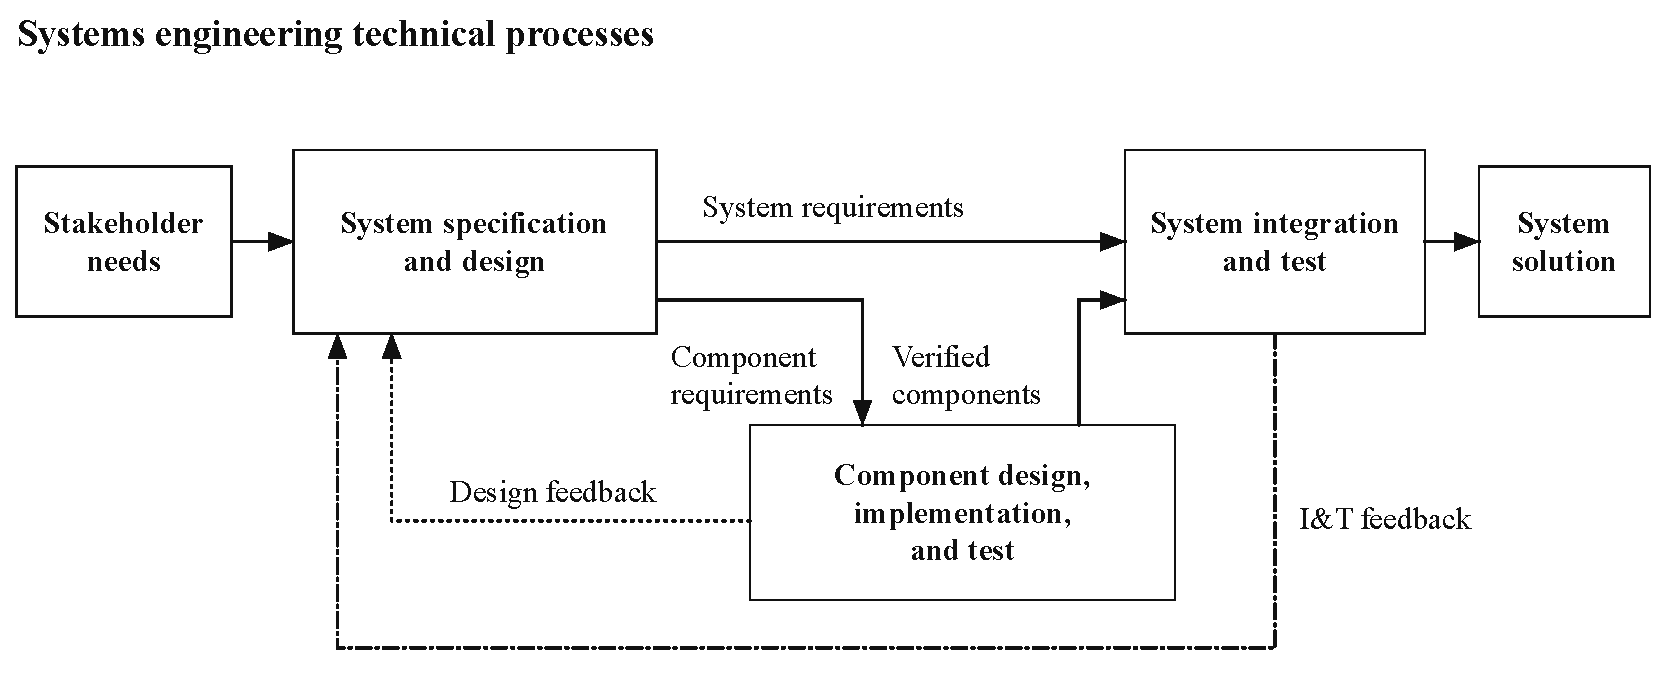
\includegraphics[width=\linewidth]{fig/systems-engineering-technical-processes.pdf}
    \caption[Simplified systems engineering technical processes.]{Simplified systems engineering technical processes. Solid arrows carry forward exchanges. Dotted arrows carry design feedback. Dash-dot arrows carry integration and test feedback. Adapted from \citet[Fig.~1.1]{friedenthal2014practical}.}
    \label{fig:systems-engineering-technical-processes}
\end{figure}

\section{Stakeholders.}
In OOSEM, a stakeholder is a person or organization with an interest in the system across its lifecycle. A stakeholder role identifies whose concerns must be addressed \citep[Secs.~17.3.2 and 17.3.5]{friedenthal2014practical}.

\section{Operational domain as-is and to-be, and enterprise.}
An operational domain provides the context for the system of interest. It contains the operational system, the users and external systems with which it interacts, and the relevant environment. An as-is domain characterizes the current context sufficiently to understand stakeholder concerns. A to-be domain describes the intended context after the mission need is addressed. Within a domain, an enterprise is an aggregation of systems and users that collaborate to achieve a set of mission objectives. It contains the system of interest and the supporting participants needed to accomplish those objectives, while other actors and environmental elements may remain external to it \citep[Sec.~17.3.2]{friedenthal2014practical}.

\section{Normative documents applicable to CUBICS proposal}
The basic normative references are the CUBICS announcements of opportunity, first released in 2022 and most recently in 2026 \citep{csa2022cubics,csa2026cubics}.
These documents define proposal eligibility and the evaluation process used to select recipients of CSA funding \citep[Secs.~3 and~5]{csa2026cubics}.
The 2022 call specified design and test reviews adapted from the NASA Systems Engineering Handbook for college and university payload or CubeSat projects \citep[App.~B.7]{csa2022cubics}. The 2026 call allows flexibility in development strategies while evaluating the documented project plan, milestones and schedule \citep[FAQ~24 and App.~C.2.1]{csa2026cubics}.
The Canadian Space Agency also published the Systems Engineering Mission Tailoring Guidelines (CSA-SE-GDL-0001), which provide guidance on tailoring systems engineering requirements by mission class, particularly for smaller Class D missions like academic nanosatellites and personnel training \citep[Secs.~1.1--1.3]{csa2020tailoring}.

By applying CSA-SE-GDL-0001 to the NASA systems engineering lifecycle, a mission treated as CSA Class D can retain the progression from concept studies through design, fabrication, integration, operations and closeout.
Engineering effort is scaled to the mission's objectives, resources and accepted risk of mission failure \citep[Secs.~3 and~3.11]{nasa2016systems}\citep[Sec.~3.2]{csa2020tailoring}.
Plans can be consolidated into a concise project plan while retaining essential requirements, interfaces, resource budgets, risks and verification evidence \citep[Sec.~3.11.4]{nasa2016systems}\citep[Secs.~4.2--4.4 and App.~B]{csa2020tailoring}.

Class D design assurance can favor commercial components, limited redundancy and fewer separate physical development and qualification units where the consequences of failure permit.
Frequent engineering discussions and peer reviews provide oversight, supported by recorded tailoring decisions, residual risks and required approvals \citep[Sec.~3.4.1]{csa2020tailoring}\citep[Sec.~3.11.3]{nasa2016systems}.

Normative documents provide requirements directly applicable to the EPS \citep[Sec.~2.3]{calpoly2022cds}.
They also constrain other subsystems, whose interfaces and operating needs lead to derived EPS requirements \citep[Secs.~4.2--4.3]{nasa2016systems}.
United Nations guidance and United States regulations provide comparative references for battery safety, passivation and disposal \citep{unoosa2010debris,fcc2026satellitecommunications}.
Canadian licensing requires five-year disposal and at least 90\% probability of disposal success \citep[Decisions~D10--D11]{ised2026debris}.

\section{Generic models of EPS requirements and architecture}
The CubeSat Design Specification and EXOpod Nova manual provide preliminary guidance on power isolation, inhibits and charging access \citep{calpoly2022cds,exolaunch2024exopodnova}.
Other subsystems contribute derived EPS requirements through their supply voltages, power consumption and operating schedules \citep[Secs.~2--4]{handpicked-0003}\citep[Sec.~2]{review-0289}.

The Object Management Group's CSRM Profile 1.1 specification complements these engineering sources with standardized categories for mission, spacecraft, subsystem and component requirements \citep[Sec.~6.1]{omg2025csrm}.
It relates requirements to the architectural elements that satisfy them and to verification activities with recorded outcomes \citep[Secs.~6.3--6.4]{omg2025csrm}.
These relationships support tracing normative and derived EPS requirements through design and verification.
The surveyed literature identifies it as mature, with 18 papers in its core research lineage covering the Radio Aurora Explorer predecessors, reference model development, and companion methods for behavior, technical measurement, validation and mission engineering \citep{review-1646,review-1621,review-1554,review-1563,review-1494,review-1487,review-1451,review-1446,kaslow2017status3,kaslow2017behaviors,kaslow2018verification,review-1288,kaslow2018status4,kaslow2019csrm,kaslow2020csrm,review-1051,kaslow2022mission,rudder2026metamodel}.

\section{Generic models of EPS components}
Luccisano et al. model shared component identity, manufacturer, mass, power by operating mode and margins per component. Their distinction between aggregate and detailed component budgets supports explicit accounting boundaries \citep[Secs.~3.1--3.2]{luccisano2024formalization}. Ceglarek and Bertrand contribute a catalog built from manufacturer datasheets with controlled parameter meanings and units. Their experience with inconsistent datasheets motivates retaining the original value and its reviewed interpretation \citep[Sec.~3]{review-0257}. The proposed schema will extend these contributions with source revisions, operating conditions, uncertainty, supported configurations and interface descriptions. These extensions will make catalog comparisons assessable.

El Hachimi et al. supply the solar maximum power point and EOL properties, battery energy and cycle-life criteria, and examples of named cells and their arrangements \citep[Secs.~3 and~6.2]{handpicked-0003}. Casado et al. contribute solar current--voltage curves with irradiance and temperature conditions, battery discharge curves and internal resistance \citep[Secs.~2.1 and~2.3]{review-0573}. Boan contributes the series/parallel configuration and mission illumination needed to assess a selected assembly \citep[Sec.~3]{review-0289}. These sources motivate separate cell and assembly records, conditional electrical characteristics and installation geometry. Wijaya et al. contribute fixed commercial product properties alongside sized alternatives. Purchased panels and packs will retain their specified dimensions, mass and ratings \citep[Sec.~III.A--B, Appendix]{review-0145}.

El Hachimi et al. contribute conditioning and bus alternatives, converter input compatibility, independently controlled outputs, protection thresholds, timing and autonomous protection functions \citep[Secs.~4 and~7.1--7.6]{handpicked-0003}. Casado et al. contribute regulator operating modes and transitions, protected output rails, and distribution efficiency estimates based on measurements \citep[Secs.~2.2 and~2.4]{review-0573}. The models will therefore distinguish conversion capabilities, electrical operating limits, loss data, channel organization and protection behavior. A controller integrated circuit record will retain its required external circuit. Its ratings alone will establish no complete converter or protected output.

In complementary approach, digital twin research supports obtaining verification evidence without fabricating the complete EPS.
Casado et al. use models validated against physical measurements to simulate EPS behavior over a complete orbital cycle \citep[Secs.~3--4]{review-0573}.
Related battery digital twin work by Zhu et al. (2025) describes virtual testing and software-in-the-loop verification without physical prototypes, followed by hardware-in-the-loop testing \citep[p.~3]{handpicked-0001}.
This is consistent with the tailored lifecycle, since NASA recognizes modeling and simulation as verification by analysis and recommends selecting methods according to project constraints and accepted risk \citep[Sec.~5.3.1.2]{nasa2016systems}.
The CSRM specification likewise includes verification under simulated or modeled conditions within its definition of analysis \citep[Sec.~6.6.8]{omg2025csrm}.
Selected requirements can therefore be verified before fabrication using credible models, while retaining the physical safety and qualification tests required by the mission and launcher \citep[Sec.~5.3.1.2]{nasa2016systems}\citep[Secs.~2.3 and~3]{calpoly2022cds}.

\section{EPS development lifecycle}
EPS development workflows link mission inputs and power budgeting to architecture, design, integration and verification within the spacecraft lifecycle \citep{handpicked-0003,review-0289}.
These workflows can be understood as an EPS development lifecycle embedded within the tailored spacecraft lifecycle, progressing from applicable normative and derived requirements to a design validated against them.
El Hachimi et al. cover the progression through functional and environmental qualification, while Boan demonstrates the preliminary stages through iterative sizing and energy balance simulations \citep[Secs.~2--5]{handpicked-0003}\citep[Secs.~2--4]{review-0289}.

Analysis of system models provides verification evidence during preliminary design.
Strobbe et al. link an EPS MBSE model to power budget calculations and propagate parameter changes to identify violated requirement constraints \citep[Secs.~III--IV]{review-0764}.
Jbara automates power and other spacecraft budget calculations and accepts or rejects candidate component selections against numerical limits \citep[Secs.~4--5]{review-0270}.
Wijaya et al. generate alternative architectures, couple subsystem sizing calculations and compare their mass, power and dimensional results with mission requirements \citep[Sec.~5.2]{review-0055}.
Their simplified sizing models support preliminary trends and relative trade-offs \citep[Sec.~6.1]{review-0055}.

  \chapter{Methodology}
\label{ch:solucion}
\hyphenrules{english}

OOSEM structures the development of the framework as the system of interest. Stakeholder analysis first allows an understanding of the as-is and to-be states of stakeholder capabilities. Then, this chapter presents the direct derivation of framework requirements, followed by their allocation to logical components and candidate physical architectures \citep[Chap.~17]{friedenthal2014practical}.

\section{Stakeholder Analysis}
The needs of stakeholders are analyzed by comparing the as-is state of their capabilities against a to-be (desired) state derived from a review of external references and the state-of-the-art.
This is a preliminary discussion that will be later formalized into verifiable requirements.
The analysis characterizes the needs, requirements, interfaces and technical criteria of nanosatellite EPS, both as observed within ASCEND and in the consulted references, and thus represents the deliverable of the first objective of this project.

\subsection{As-is capabilities}
For the CUBICS mission, a collaboration between ASCEND researchers and members of a student club at ÉTS is being proposed.
The present work is aimed at serving them both.

ASCEND researchers are familiar with systems engineering and even MBSE, but the nature of their position does not allow them to contribute significant time to the practical aspect of CubeSat design and development.
In contrast, ASCEND-associated students who wish to participate in CUBICS have years of experience in building systems for student engineering competitions but follow no systems engineering method.

The students have built CubeSat-format payloads for rocketry competitions, for which they verified payload power requirements only after fabrication.
This verification was observed to take the form of reusing a legacy battery pack for which the original calculations have been lost, connecting all loads, and performing mission operations repeatedly until the stored energy was depleted.
If the time until energy depletion was greater than the duration of one operations cycle as defined by the competition rules, the power requirements were taken as verified.
These experiments were reported to result in battery lifespans several times greater that one operations cycle, with the students opining that the battery pack was oversized.

In contrast, the student club members have ample experience in verifying requirements related to rocket mass, maximum height, and maximum speed before fabrication, via inspection and analysis in simulation.
These requirements are given as numerical targets by each rocketry competition, or derivated from the top-place results of previous competitions.
These competition requirements are always expressed in terms of measurable quantities, which is essential for competition grading.

ASCEND researchers report an EPS design that has been in progress for nine months.
Unclear definition of requirements has been a recurring issue, and it has forced redesigns when it is discovered that the existing requirement list is incomplete.
Requirement changes force the researchers to wait at least one week, until the next one hour-long weekly meeting, to assess their impact, because the traceability from requirements to design has to be established manually each time.

\subsection{Stakeholder concerns}
\label{sec:stakeholder-concerns}

Following OOSEM, stakeholder discussions identified concerns about the cost and effort of closing capability gaps.
These concerns inform framework requirements and measures of performance.

A project manager and systems engineer at ASCEND is concerned with maintaining verifiable requirements, redesign after fabrication, and tools suited to the team's mission scale and resources \citep[Secs.~4--5]{handpicked-0003}\citep[Sec.~1]{review-0573}\citep[Sec.~5.1]{buruso2026modelbased}.
That stakeholder is also concerned with requirement traceability, communicating verification and validation evidence, and updating EPS and other subsystem power requirements as designs change.
Maintaining consistency across requirements, models and verification evidence also demands effort \citep[Secs.~4.4 and~5.1]{buruso2026modelbased}\citep[Secs.~3--4]{review-0853}\citep[Sec.~V]{citation-0136}.

An EPS engineer is concerned with repeating verification after requirement changes, tracing design decisions, revising designs after failed verification, updating component requirements and communicating designs during technical reviews.
Further concerns include verifying safe and effective charging and power management \citep[pp.~1--3 and~6]{handpicked-0001}\citep[Sec.~3]{handpicked-0003}\citep[Secs.~5.1 and~6]{review-1251}.
Engineers responsible for other subsystems share the concern about verification cost and effort.

Taken together, the aforementioned as-is capability gaps and associated concerns can be formulated as a problem that motivates the current project:

\begin{quote}
Evidence fragmentation during the early lifecycle phases of nanosatellite electrical power systems hinders the traceability between needs and requirements, architecture decisions, and the analytical evidence that supports them. Furthermore, it hinfers the reproducibility of analyses and the capability to detect design inconsistencies before advacing to physical verification and validation phases.
\end{quote}

\subsection{Potential to-be capabilities}
After observing as-is stakeholder capabilities and recording them objectively, the OOSEM method suggests analyzing the capabilities of existing external enterprises and systems. From this, capability gaps or the lag behind the state-of-the-art can be identified and later formalized into the requirements for the systems and processes that will improve these capabilities, in this case the proposed framework.
Sources for this comparison include the academic literature, crucial for ASCEND as a research group, and normative documents.
Said sources were discussed amply in Chapter \ref{ch:marco}, to which the reader is referred in order to avoid repetition.

\section{System Requirements Analysis}
\label{section:analyze-system-requirements}
System Requirements Analysis defines how the to-be (desired) stakeholder capabilities can be obtained with support from the system of interest, the framework in this case.
The requirements define what the framework must accomplish for the stakeholders constrained by acceptable ranges of measurable system variables (Measures of Performance in OOSEM), which make them verifiable.

Table~\ref{tab:framework-requirements} gives the full list of framework requirements.
FR-01 and FR-02 establish the base unit of engineering knowledge as a requirement with forward and reverse links and quantitative values, which are used in MBSE approaches to construct a model representation of the mission.
FR-06 enables the capability to assess the impact of a change in a quantitative requirement, which is desired by the stakeholders in order to explore alternatives and keep requirements up to date in an agile manner.
FR-03 establishes that whenever an analysis is executed its inputs and outputs have to be contextualized by the mission requirements.
FR-09 establishes a controlled evolution of mission requirements and the architecture choices that depend on them, while FR-04 specifies that this evolution must be replicable without loss of information.

FR-07 and FR-08 aim to lessen the workload of inexperienced engineers, who understand EPS development from technical specifications but may struggle to follow a systems engineering line of work from high-level mission requirements, with the necessary verification measures at every step.
FR-10 and FR-11 support progress along the EPS engineering lifecycle, where early designs with ideal or assumed values must mature into evaluating the properties of real COTS.
FR-05 states that the model of what an EPS consists of, which delimits which COTS are relevant for this framework within the inmense entirety of commercial offerings, must adhere to the CSRM Profile 1.1 specification.

FR-12 to FR-20 cover fundamental analyses that are considered in the literature to be the minimum set that verifies an early EPS design and the COTS choices made for it from Phase 0 to Phase B in the NASA Reference Lifecycle. This is what the problem statement of this projects refers to as early lifecycle phases.
They cover the component types defined by CSRM and common tradeoff analyses performed at this level of design maturity.

{\small
\setlength{\tabcolsep}{4pt}
\setlength{\parskip}{0pt}
\setlength{\LTpre}{0.4\baselineskip}
\setlength{\LTpost}{0.4\baselineskip}
\renewcommand{\arraystretch}{1.06}
\begin{longtable}{@{}>{\raggedright\arraybackslash}p{0.08\linewidth}>{\raggedright\arraybackslash}p{\dimexpr0.92\linewidth-2\tabcolsep\relax}@{}}
\caption{Framework requirements.}\label{tab:framework-requirements}\\
\toprule
\textbf{ID} & \textbf{System requirement} \\
\midrule
\endfirsthead
\toprule
\textbf{ID} & \textbf{System requirement} \\
\midrule
\endhead
\bottomrule
\endfoot
FR-01 & The framework shall retain each requirement with its identifier, statement, parents and children, rationale, conditions or quantities, applicable units, verification method, and resolution status, including reasons for unresolved fields. \\
FR-02 & The framework shall retain forward and reverse links among requirements and component allocations. \\
FR-03 & The framework shall associate each analysis result with its requirement/expectation, method, scenario, parameters, raw outputs, and execution status. \\
FR-04 & The framework shall provide the inputs, dependencies and instructions to reconstruct all analyses of a mission. \\
FR-05 & The framework shall allocate EPS requirements among components covering generation, storage, conversion, regulation, protection, distribution, and control components as per the CSRM Profile 1.1 specification. \\
FR-06 & The framework shall identify impacts of a proposed mission, requirement, component, or model change on requirements and EPS design. \\
FR-07 & The framework shall recommend next engineering activities and from the current activity and inputs. identifying unmet prerequisites. \\
FR-08 & The framework shall recommend analysis, verification and validation methods or models on edits or requests using available inputs. \\
FR-09 & The framework shall retain retrievable mission states that resolve exact requirement, mission, design, and model revisions with revision history and the authorized decisions that control them. \\
FR-10 & The framework shall estimate electrical and dynamic EPS model parameters from quality-checked data. \\
FR-11 & The framework shall propose COTS EPS components from available requirements. \\
FR-12 & The framework shall calculate EPS mass and occupied volume estimates from aggregate or component data and assess margins against allocations, retaining sources, units, and unknown values. \\
FR-13 & The framework shall retain mission orbit, attitude, duration, environmental conditions, subsystem modes, and load schedules as inputs to EPS requirements and analysis. \\
FR-14 & The framework shall calculate mode-dependent power, sunlight/eclipse energy budgets, and beginning/end-of-life array and battery sizing, reporting integer cell counts, array area, and battery capacity. \\
FR-15 & The framework shall compare EPS concepts and architectures through common feasibility checks covering different choices of cell technology, reporting raw measures and unknown values. \\
FR-16 & The framework shall compare EPS concepts and architectures through common feasibility checks covering different choices of array/battery series and parallel configurations, reporting raw measures and unknown values. \\
FR-17 & The framework shall compare EPS concepts and architectures through common feasibility checks covering different choices of bus voltage and buck/boost regulation, reporting raw measures and unknown values. \\
FR-18 & The framework shall execute EPS analyses covering photovoltaic I--V/P--V characteristics against available electrical and component-rating limits. \\
FR-19 & The framework shall execute EPS analyses covering direct energy transfer vs. MPPT, against available electrical and component-rating limits. \\
FR-20 & The framework shall execute EPS analyses covering overcurrent/undervoltage/overvoltage cases. \\
\end{longtable}
}

\subsection{Measures of performance}
\label{subsection:framework-mops}

Table~\ref{tab:framework-mop-protocols} assigns Measures of Performance to the framework requirements \citep[Sec.~17.3.3]{friedenthal2014practical} to make them verifiable.
Each MOP is evaluated through one of two verification scenarios.

The first scenario reconstructs every power budget in the BIRDS-4 presentation \citep[pp.~5, 8--9, 13, 15]{shrestha2022birds4powerbudget} and the September 2019 OreSat budget \citep{oresat2019powerbudget}. The publications cited in Table~\ref{tab:framework-mop-protocols} extend these cases with mass budgets, COTS selection criteria, architecture trades, measured solar characteristics and protection tests. Each MOP in this scenario is evaluated separately for BIRDS-4 and OreSat using each mission's own published conditions. Both missions must satisfy its desired range for the MOP to pass.

For FR-12 to FR-20, expected numerical results and findings come directly from the cited publications. For each nonzero reference value $r$, the framework output $x$ must satisfy $|x-r|/|r|\leq 0.01$ after unit conversion. This 1\% tolerance applies to every numerical comparison in each mission separately. Results are not averaged across outputs or missions. Zero references require zero outputs. Component counts, series/parallel arrangements, and categorical findings require exact agreement with their references. Missing outputs fail the comparison. Source inconsistencies are reported without changing the published values.
% A missing published reference for either mission leaves that mission's comparison unverified. Evidence from the other mission does not complete the MOP.

The second scenario consists of two individual user trials, one with a PhD candidate from ASCEND and one with an undergraduate from the student club. Each participant completes the three GUI tasks in Table~\ref{tab:framework-mop-protocols} from prepared initial states. Each trial lasts 60~min, divided equally among the tasks. An evaluator prepares the task inputs and reference answers before the trials. Each GUI MOP measures elapsed time from task presentation until the saved changes and reported results match these references. Both participants must complete each task within 20~min. Incorrect or unfinished tasks are recorded as unsuccessful.

\begingroup
\small
\setlength{\tabcolsep}{4pt}
\setlength{\parskip}{0pt}
\setlength{\LTpre}{0.4\baselineskip}
\setlength{\LTpost}{0.4\baselineskip}
\renewcommand{\arraystretch}{1.0}
\setlength{\ReportTableBodyWidth}{\dimexpr\linewidth-4\tabcolsep\relax}
\begin{longtable}{@{}P{0.20\ReportTableBodyWidth}P{0.60\ReportTableBodyWidth}P{0.20\ReportTableBodyWidth}@{}}
\caption{Framework measures of performance.}\label{tab:framework-mop-protocols}\\
\hline
\textbf{MOP/FR} & \textbf{Verification protocol} & \textbf{Desired range} \\
\hline
\endfirsthead
\hline
\textbf{MOP/FR} & \textbf{Verification protocol} & \textbf{Desired range} \\
\hline
\endhead
\hline
\endfoot
\multicolumn{3}{@{}l}{\textbf{BIRDS-4 and OreSat case studies and catalogue inspection}} \\*
MOP-02/FR-02 & Retrieve forward and reverse links among the mission requirements and component allocations. Compare all linked requirement and component identifiers with the prepared mission references. & 100\% correct links \\
MOP-03/FR-03 & Inspect every budget run, including a deliberately failed run, for its linked requirement, method, scenario, parameters, available raw outputs and execution status. Compare retained records with the executed cases. & 100\% correct result records \\
MOP-04/FR-04 & Use each mission's retained inputs, dependencies and instructions to independently reconstruct and rerun all analyses in a fresh environment. Compare every output with the saved run and the applicable published reference. & $\leq 1\%$ deviation\newline All analyses reconstructed \\
MOP-05/FR-05 & Allocate each mission's EPS requirements to its catalogue components across the seven FR-05 functions. Compare component identifiers, CSRM Profile 1.1 types and allocation links with the prepared references. & 100\% correct allocations \\
MOP-06/FR-06 & Change a mission input, a requirement limit, a component and a model parameter separately. Compare affected requirement/design identifiers and updated budgets with independent dependency and calculation references. & $\leq 1\%$ deviation\newline 100\% correct impacts \\
MOP-09/FR-09 & Save both mission baselines with their revision and authorized decision records, then modify inputs and allocations. Retrieve each baseline and compare requirement, mission, design and model revisions and decision histories with the saved references. & 100\% correct baseline records \\
% FR-10: catalogue inspection verifies sourced data, not parameter estimation or dynamic model accuracy.
MOP-10/FR-10 & Present the COTS database, including components from both missions, as a table of part numbers, parameters, units, operating conditions and links to the manufacturer datasheets. Inspect each populated value against its cited page, table or curve. & 100\% correct, traceable values for both missions \\
MOP-11/FR-11 & For each mission, supply the documented selection criteria without the selected part numbers. Compare recommendations with BIRDS-4's LTC3119 choice \citep[p.~1025]{kim2021birdsbus} and OreSat's Tenergy 30005-0 and MAX17205 choices \citep{greenberg2021oresat,oresatbatteryresearch,oresat2025batterydesign}. Accept the original choice or an alternative that satisfies every documented constraint and improves the stated quantitative selection measure. & $\geq 1$ candidate per selection in each mission\newline 100\% of criteria satisfied \\
% FR-12: the OreSat budget supplies EPS subassembly masses. Its complete spacecraft mass is not an EPS mass reference.
% Published aggregate EPS mass, occupied volume and margin references remain incomplete for both missions. BIRDS-4 has no sourced aggregate EPS mass case in the selected publications.
% The 2016 OreSat mass budget also contains inconsistent line sums and an approximate spacecraft margin. Preserve these source discrepancies.
MOP-12/FR-12 & For both missions, calculate EPS mass, occupied volume and margins against allocations. Compare each result with a published reference at the same component boundary, including OreSat's 252~g solar module and 416~g battery module entries \citep[Sec.~D.2]{oresat2016csli}. Check retained sources, units, unknown values and margin findings for each mission. & $\leq 1\%$ per mission\newline Exact records and findings \\
MOP-13/FR-13 & For BIRDS-4 and OreSat, enter and save orbit, attitude, duration, environment, modes and load schedules from their published mission records \citep{jara2022birdsepsdataset,oresat2019powerbudget}. Reopen each mission and compare retained fields and analysis inputs with its own source values. & $\leq 1\%$ per mission\newline Exact categorical inputs \\
% FR-14: the budgets verify reported energy and storage calculations. Full mission BOL/EOL array and battery sizing and installed array area lack published output references for both missions.
MOP-14a/FR-14 & Recalculate all published load and generation rows, mode totals, storage capacities, battery configurations, recharge times and payload pass counts for both missions using their original quantities, duty cycles and margins. Compare every output separately with its mission's published value. & $\leq 1\%$ per mission\newline Exact counts and arrangements \\
MOP-14b/FR-14 & Reproduce the BIRDS-4 worst-case budgets with 1604, 1202 and 801~mWh available at the load and the deficit against 1438~mWh nominal consumption \citep[Tables~2--4]{shrestha2022birds4powerperformance}. Reproduce OreSat's 1011~mWh standby energy surplus \citep{oresat2019powerbudget}. Compare energy quantities and balance findings separately for both missions. & $\leq 1\%$ per mission\newline Exact published findings \\
% FR-15: the 2026 BIRDS-4 hybrid result is a proposed configuration simulated with sun tracking, not a flown BIRDS-4 configuration or its original free-rotation budget.
% The article also mentions free rotation and gives a generic physical-parameter table from a 6U study. Resolve the applicable published inputs before claiming 1% reproduction of its BIRDS-4 result.
MOP-15/FR-15 & Compare published cell technology alternatives for both missions. Reproduce the BIRDS-4 hybrid solar case with ten triple-junction and six monocrystalline cells and 3.023~Wh per orbit \citep[Sec.~III]{shrestha2026solarreliability}. Repeat OreSat's lithium-ion, lithium iron phosphate and lithium titanate trade \citep{oresatbatteryresearch}. Compare each mission's energies, capacities and selection findings under its published conditions, retaining unknown properties. & $\leq 1\%$ per mission\newline Exact published findings \\
% FR-16: BIRDS-4 baseline arrangements are sourced. Published alternative arrangement cases and their feasibility findings remain needed for complete BIRDS-4 comparison coverage.
MOP-16/FR-16 & For each mission, compare array and battery series/parallel choices with published counts, capacities and selection findings. Include BIRDS-4's two-cell solar strings and 3S2P, 3800~mAh battery \citep[Sec.~2.2, Table~5]{shrestha2021birdssafety}, OreSat's two independent 2S packs and 37.4~Wh per card \citep[p.~6]{greenberg2021oresat}, and its 74.88, 86.4 and 64.8~Wh alternatives against 80~Wh \citep{oresatbatteryresearch}. & $\leq 1\%$ per mission\newline Exact counts, arrangements and findings \\
MOP-17/FR-17 & For each mission, compare bus voltage intervals, buck/boost functions and feasibility findings with published cases. Check BIRDS-4's 3.3 and 5~V regulated lines \citep[Sec.~2.2.3]{shrestha2021birdssafety} and OreSat's 1S, 2S and 4S bus choices and SPV1040 rejection after the change from 1S to 2S \citep{oresatbatteryresearch,oresatsolarhistory}. & $\leq 1\%$ per mission\newline Exact published findings \\
% FR-18 compares labelled graph values and published spreadsheet outputs. Unlabelled coordinates do not receive an assumed 1% reading accuracy.
% Empirical I--V samples support numerical reconstruction. Reusing those samples as both model inputs and prediction references does not validate a physical cell model.
MOP-18/FR-18 & Reconstruct the BIRDS-4 Maya-2 +Z panel I--V/P--V characteristics and compare labelled voltages, powers and the 1.575~W peak with the published curves \citep[Figs.~13--14]{shrestha2021birdssafety}. Reconstruct OreSat's measured solar sweep and compare calculated power with its published spreadsheet values \citep{oresatsolarsweep}. Check each mission's labelled or tabulated values separately. & $\leq 1\%$ per mission \\
% FR-19: no published paired DET/MPPT case was found for either mission. Both missions still need sourced numerical cases for this MOP.
% BIRDS fixed input-voltage control and OreSat's regulated constant-voltage fallback are not DET references.
MOP-19/FR-19 & For BIRDS-4 and OreSat separately, compare DET and MPPT using published paired cases with identical array, battery, illumination and load conditions. Compare delivered energy, operating points, conversion losses and electrical-limit findings with that mission's published results. & $\leq 1\%$ per mission\newline Exact published findings \\
% FR-20 checks steady-state overvoltage protection, static currents, protection settings and state logic. A published BIRDS-4 undervoltage protection case is still missing, and these sources do not establish transient fault response accuracy for either mission.
MOP-20/FR-20 & For both missions, check overcurrent, undervoltage and overvoltage cases against published outputs and protection findings. Include BIRDS-4's BCR test with input at or above 4.8~V and output near 4.2~V \citep[Sec.~3.6]{shrestha2021birdssafety} and its 2, 3 and 4~A line thresholds \citep[Sec.~6.3]{kyutech2021birdsicd}. Check OreSat's 30~W load currents and charge/discharge disable and recovery criteria \citep{oresat2025batterydesign}. & $\leq 1\%$ per mission\newline Exact published protection findings \\
\multicolumn{3}{@{}l}{\textbf{User trials}} \\*
MOP-01/FR-01 & Given a fully defined mission requirement, create another requirement with the FR-01 fields filled in and a simple verification condition, reopen it, and report its retained fields and condition result. & $\leq 20$~min \\
MOP-07/FR-07 & Given complete mode allocations and load powers with eclipse duration omitted, request the next activity and identify the unmet prerequisite. Supply that duration and report the updated recommendation. & $\leq 20$~min \\
MOP-08/FR-08 & Given an EPS requirement and its supporting inputs, request analysis, verification and validation recommendations and report the suggested methods or models. & $\leq 20$~min \\
\end{longtable}
\endgroup

\section{Define Logical Architecture}
\label{section:define-logical-architecture}

Nine logical components realize F01--F08 without specifying implementation technologies \citep[Sec.~17.3.4]{friedenthal2014practical}. Learning, finances, RAM, credibility, software and technician concerns extend the response beyond evidence custody. El Hachimi et al. inform mission-driven sizing, component and thermal/EMC decisions, protection and telemetry checks \citep[Secs.~2--5 and~8.1.6--8.1.7]{handpicked-0003}. The Handbook informs coordinated requirements, budgets, interfaces and verification planning \citep[Secs.~I.3--I.4]{aguado2021cubesatse}. Their EPS results remain case-specific.

\subsection{Responsibilities and allocations}

Figure~\ref{fig:framework-logical} presents three views of the same nine logical components, with their important records, required information and provided services. Each dashed reference refers to an existing component, not an additional component or deployment. FR numbers identify the 40 primary responsibility allocations. Supporting responsibilities and exchanges remain formalized in the SysML v2 model. This decomposition imposes no executable or node count. Intended allocation is not demonstrated requirements satisfaction \citep[Sec.~17.3.7]{friedenthal2014practical}.

% One figure, continued across three pages to keep the native summaries readable.
\begin{figure}[p]
\centering
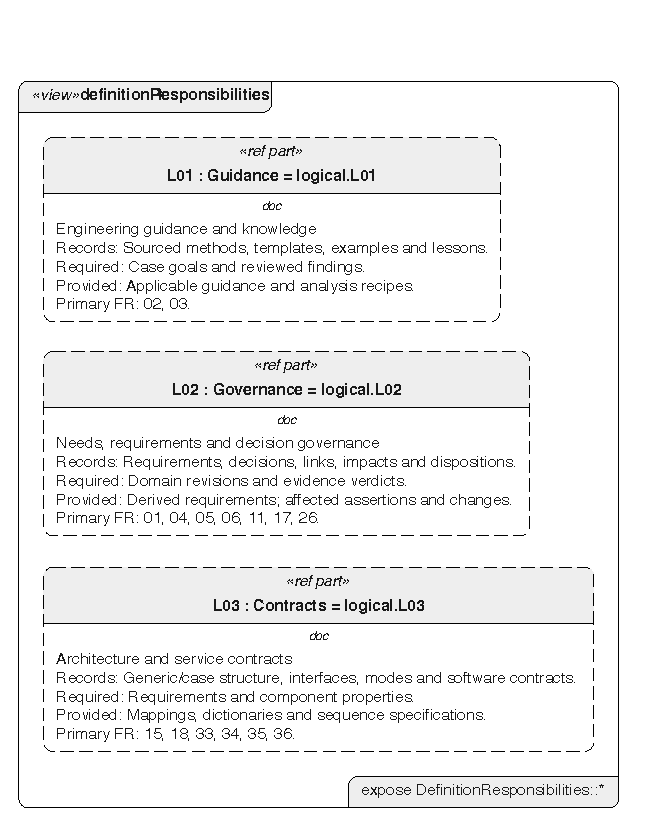
\includegraphics[width=\linewidth,height=0.84\textheight,keepaspectratio]{fig/sysml/logical/sysml-defined-view-logicalresponsibilityviews-definitionresponsibilities.pdf}
\caption{Logical component responsibilities, records and required/provided services. Primary FR numbers state intended allocation, not demonstrated satisfaction. (a) L01--L03: guidance, governance and architecture.}
\label{fig:framework-logical}
\end{figure}
\begin{figure}[p]
\ContinuedFloat
\centering
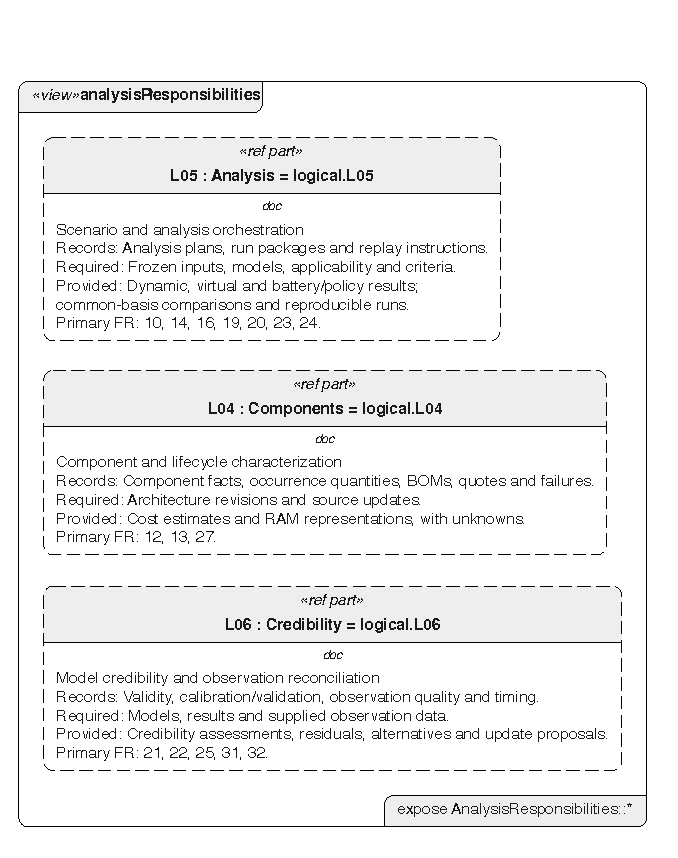
\includegraphics[width=\linewidth,height=0.84\textheight,keepaspectratio]{fig/sysml/logical/sysml-defined-view-logicalresponsibilityviews-analysisresponsibilities.pdf}
\caption[]{Logical component responsibilities (continued). (b) L04--L06: characterization, analysis and credibility.}
\end{figure}
\begin{figure}[p]
\ContinuedFloat
\centering
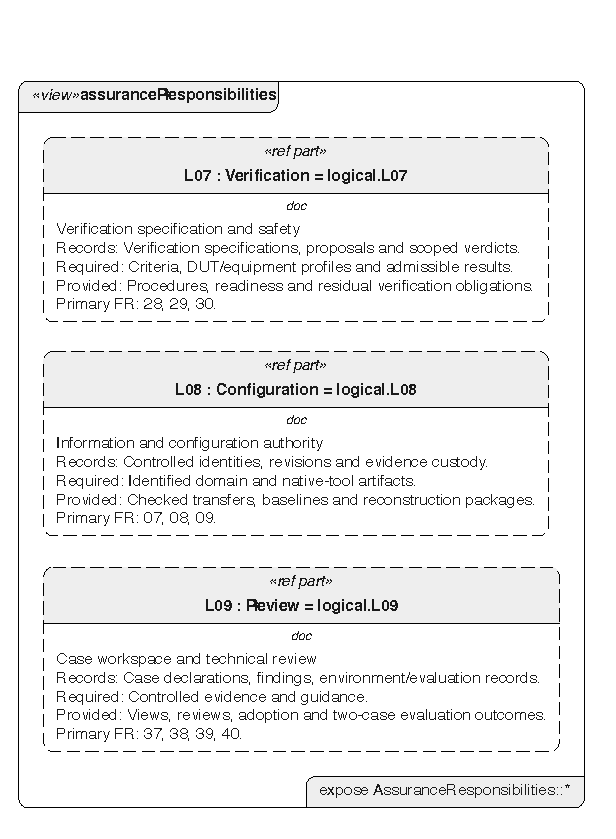
\includegraphics[width=\linewidth,height=0.84\textheight,keepaspectratio]{fig/sysml/logical/sysml-defined-view-logicalresponsibilityviews-assuranceresponsibilities.pdf}
\caption[]{Logical component responsibilities (continued). (c) L07--L09: verification, configuration and review.}
\end{figure}
\clearpage

\subsection{Typed exchanges, authority and feedback}
{\small
\setlength{\tabcolsep}{4pt}
\setlength{\parskip}{0pt}
\setlength{\LTpre}{0.4\baselineskip}
\setlength{\LTpost}{0.4\baselineskip}
\renewcommand{\arraystretch}{1.06}
\begin{longtable}{@{}>{\raggedright\arraybackslash}p{\dimexpr0.32\linewidth-0.64\tabcolsep\relax}>{\raggedright\arraybackslash}p{\dimexpr0.68\linewidth-1.36\tabcolsep\relax}@{}}
\caption{Information exchanges between logical components.}\label{tab:framework-logical-exchanges}\\
\toprule
\textbf{Participants} & \textbf{Exchanged information and required handling} \\
\midrule
\endfirsthead
\caption[]{Information exchanges between logical components. (continued).}\\
\toprule
\textbf{Participants} & \textbf{Exchanged information and required handling} \\
\midrule
\endhead
\bottomrule
\endfoot
All $\leftrightarrow$ L08 & Registration, transfer verdict, exact manifest and reconstruction. Check envelope/semantics/provenance and preserve rejected/prior revisions. \\
L02 $\leftrightarrow$ L03/L04/L06/L07 & Requirements, criteria, impact and domain revision proposals. Resolve dependencies and retain stale/unresolved evidence. \\
L03/L04/L06/L07 $\rightarrow$ L05 & Occurrences, characterization, failure dependencies, applicable models and verification criteria freeze the run. Software mappings also drive sequence/resource checks. \\
L05 $\rightarrow$ L06 $\rightarrow$ L07 $\rightarrow$ L02 & Raw analysis results, model credibility assessment, verification verdict based on admissible evidence and status of affected technical assertions. Supplied observations return through proposed parameter/design updates. \\
L01/L09 $\leftrightarrow$ domain owners & Guidance, baseline-linked reviews, findings and lessons. Apply tailoring, return findings to owners and separate local learning from general source claims. \\
\end{longtable}
}

L08 controls accepted baselines and consistent identification. Each domain component remains responsible for the meaning of its information: requirements (L02), architecture and interfaces (L03), component characteristics (L04), models and observations (L06), verification (L07), knowledge (L01) and case reviews (L09). Generated analysis inputs, software definitions and views refer to these controlled sources rather than creating competing definitions. Mission software behavior and deployment still require separate implementation and verification \citep[Secs.~3--5]{review-0853}.

Interface specifications for quantities, signs, reference frames, clocks and validity address model, degradation, sensor and timing effects \citep[Secs.~4.1--4.2 and~6]{review-1251}. Numerical step size proves no real-time suitability \citep[Sec.~3]{review-0573}. SC01 follows guidance and definition, analysis, credibility assessment, verification and review. SC02 evaluates change impacts through domain revisions and reanalysis. SC03 uses failed checks or supplied observations to propose updates and safe verification activities. Design change, observation reconciliation and reviewed learning share L08 revision control. They never silently overwrite earlier evidence or actuate hardware.

\section{Synthesize Candidate Physical Architectures}
\label{section:synthesize-physical-architectures}

The physical architecture identifies the software, persistent data, operating procedures and computing resources that realize the eight logical responsibilities. OOSEM first partitions responsibility, information and control across logical nodes. It then allocates them to physical components and hosts, with explicit interfaces and component specifications \citep[Sec.~17.3.5]{friedenthal2014practical}. This is the framework architecture. EPS arrays, batteries, converters and controllers remain engineered model/software products.

\subsection{Partitioning and common scope}

Three logical nodes group the current responsibilities. The \emph{engineering node} contains exchange, requirements, design, analysis, credibility and review (L01, L03--07). The \emph{assistance node} contains L02. The \emph{evidence node} contains configuration and currency (L08). These groups separate interactive drafting from long numerical work and separate editable working records from preserved releases. They describe responsibilities rather than a fixed number of computers.

{\small
\setlength{\tabcolsep}{4pt}
\renewcommand{\arraystretch}{1.06}
\begin{longtable}{@{}>{\raggedright\arraybackslash}p{0.30\linewidth}>{\raggedright\arraybackslash}p{\dimexpr0.70\linewidth-2\tabcolsep\relax}@{}}
\caption{Physical partition decisions and their measures.}\label{tab:framework-partitioning}\\
\toprule
\textbf{Criterion} & \textbf{Consequence and current basis} \\
\midrule
\endfirsthead
\toprule \textbf{Criterion} & \textbf{Consequence and current basis} \\
\midrule
\endhead
\bottomrule
\endfoot
Meaning and authority & Keep requirement, design and evidence meanings with L03, L04 and L06--07. L08 preserves their exact revisions. Assign one owner per field. MR-02--05, MOE-02--03, MOP-03--05. \\
Interactive response & Run assistance independently of numerical execution. Invalidate guidance immediately on edits. Record pending/unavailable work. MR-02 and 05, MOE-01 and 04, MOP-01--02 and 04. \\
Replaceable analysis & Declare discipline, model, solver and host profiles at the analysis boundary. Verify every mandatory profile. Separate execution from credibility and EPS assessment. MR-03--04, MOE-02--03, MOP-03 and 05. \\
Access and preservation & Keep private engineering inputs local by default. Preserve sources, raw results and released dependencies with backup/restore. Verify external access, exports and recovery. MR-05, MOE-03--04, MOP-04--06. \\
Adoption and variation & Separate reusable rules, libraries and methods from mission inputs and model/software products. Compare correct-task effort and dated framework cost. MR-01--05, MOE-01 and 04, MOP-06. \\
\end{longtable}
}

Every complete candidate specifies the same 41 FRs, eight logical responsibilities and Pre-Phase A through adapted C tasks. Each includes active drafting assistance, explained contextual recommendations, EPS modeling, applicable discipline/RAM analysis, credibility, controlled changes and reviews. An external declared host toolchain codes, builds and executes SIL only after the exact current engineer-authorized detailed design/interface release. Generic computing hosts are framework infrastructure. Physical EPS realization, procurement, testing, PIL/HIL and flight readiness remain excluded.

\subsection{Five coherent configurations}

Five configurations provide distinct authoring and collaboration arrangements. These are COMET and Excel (PA-COM), SysML and Python (PA-CDT), YAML and Git (PA-GY), Nanospace (PA-NS), and Capella and Valispace (PA-VS). Shared proposed assistance and analysis components make their scope comparable. Source-supported workflows establish reusable mechanisms. They establish neither complete EPS readiness nor implemented framework compliance.

{\small
\setlength{\tabcolsep}{4pt}
\renewcommand{\arraystretch}{1.07}
\begin{longtable}{@{}>{\raggedright\arraybackslash}p{0.14\linewidth}>{\raggedright\arraybackslash}p{\dimexpr0.43\linewidth-2\tabcolsep\relax}>{\raggedright\arraybackslash}p{\dimexpr0.43\linewidth-2\tabcolsep\relax}@{}}
\caption{Five complete candidate configurations. All additions require development and verification.}\label{tab:framework-candidate-inventories}\\
\toprule
\textbf{Candidate} & \textbf{Configuration and reason to retain} & \textbf{Proposed additions and important limits} \\
\midrule
\endfirsthead
\toprule \textbf{Candidate} & \textbf{Configuration and reason to retain} & \textbf{Proposed additions and important limits} \\
\midrule
\endhead
\bottomrule
\endfoot
PA-COM & COMET server, desktop client and Excel add-in provide parameter ownership, catalogues and budget calculations. Retain this concurrent engineering arrangement \citep[Secs.~3--4]{deutsch2022comet}. & Python companion requirement/trace records, edit-linked assistance, analysis, credibility, reviews and Git/archive releases. COMET parameters are linked to requirement meaning. Current API/add-in compatibility, Excel rights and workbook reconstruction are unresolved. \\
PA-CDT & Native SysML v2 authoring and views through Syside, Python engineering calculations, Git and a managed archive. Retain explicit local model authority and replaceable tools. CSRM supplies structural patterns \citep{kaslow2019csrm}. & A native EPS library, authoring assistance panel, analysis/profile mappings, impact checks and assessment services are proposed. CSRM is not a completed SysML v2 migration. Deployment licence, authoring API, quantities, capacity and clean reconstruction need proof. \\
PA-GY & Typed YAML engineering definitions, Git review, an editor/Python assistance panel and generated views. Retain portable reviewable text \citep{kanavouras2024lightweight,chiu2023sealion}. & Develop engineering units/relationships, requirement allocation, assistance, analyses, credibility and authority controls. The lightweight source excludes requirement/test management. Git history supplies no technical approval. Contributor usability is unresolved. \\
PA-NS & Nanospace browser/API parameter collaboration, declared native model authority, Python services and Git/archive releases. Retain concurrent sharing and dependency analysis \citep[Secs.~3--6]{review-0340}. & Add active browser assistance, requirement semantics, controlled exports and full analysis/assessment services. HyperTension/HDDL planning is an optional proposed adapter. Integrated planning is future work. Gaphor extraction is a separate tool-specific option \citep{luccisano2024formalization}. \\
PA-VS & Capella/ARCADIA owns structure, allocations, modes and interface meanings. Valispace owns requirements, properties and budgets. Python for Capella and REST transfers connect them \citep[Secs.~3--4]{campioli2025integration}. & Add edit-linked assistance, stable-ID reviewed transfers, dynamic analysis, credibility and Git/archive releases. Demonstrated preliminary tree/mode/budget transfers support retention. Current service access, deletion/conflict handling, exports and reconstruction remain unresolved. \\
\end{longtable}
}

Each candidate deploys its engineering services on a generic workstation and any declared authoring server, local assistance on an independently scheduled process, and identified releases/raw outputs on a managed archive. These roles can share hardware if access, response, numerical workload and recovery limits are met. Versions, CPU, memory, storage, network, operating system, licences and backup arrangements must be declared before deployment. No capacity or licence price is assumed.

\subsection{Active assistance realization}
\label{subsection:physical-assistance}

The service retrieves relevant engineering sources, ranks candidate findings or methods, and prepares cited explanations for engineer assessment.

Every candidate includes the following proposed Python service. Its attachment point is the COMET/Excel editor, native model workbench, YAML editor, Nanospace browser or Valispace/Capella workspace. An edit is acknowledged and invalidates affected current and pending guidance before delayed work starts. The service captures the exact requirement, mission, design, source, criterion and scope revisions.

\paragraph{Rules, selection and ranking.}
Versioned structural, quantity and wording rules check required fields, identifiers, parents, responsible product, modal wording, single obligations, units, inequalities and declared numerical limits. NASA Appendix C and an expert-approved project reference supply the default criteria \citep[Sec.~4.2 and Appendix~C]{nasa2016systems}. Broad semantic findings remain probable. For example, ``battery capacity: 200 W'' triggers a dimensional finding and a question about the intended quantity. It cannot justify inventing ``200 Wh''.

Source selection preserves authority and citation metadata while selecting substantive passages, tables, equations and necessary context. BM25 retrieves candidate passages through lexical ranking against the query terms. Local \texttt{Qwen3-Embedding-0.6B} retrieves semantic candidates, and \texttt{Qwen3-Reranker-0.6B} scores query/passage pairs \citep{qwen3embedding,qwen3reranker}. Their proposed initial revisions are respectively \texttt{97b0c614be4d} and \texttt{e61197ed4502}. The native specification retains the full revisions. Tokenizer, prompts, library versions and input limits also require control. Separate content and contextual relevance rubrics require qualification. Necessary standards passages cannot disappear silently through a content filter.

Pinned \texttt{jev-1.13.0} through TypeSafe SDK 0.6.0 is an alternative for substantive-content and current-question relevance scoring \citep{typesafe060}. Structured requirement-pair similarity/conflict questions are a proposed additional use. Existing passage reranking is pointwise. Noul scores return neither explanations nor corrections. Requested and returned model identities must agree with the qualified profile. A changing ``latest'' alias is excluded. Local Qwen/BM25 offers data locality and offline operation, with resource and domain-qualification costs. Jev offers an external scoring service, with unresolved access, privacy, cost, outage and qualification dependencies. Neither option demonstrates technical correctness.

Method/model options first pass mandatory scope, purpose, input, fidelity, validity, resource and access checks. Unknown prerequisites remain unresolved. Only eligible options enter shortlist ranking. Duplicate candidates compare level, subject, mode, conditions, quantity and parent allocation. Similar statements can be valid separate requirements. Coverage uses a declared ConOps/function/interface/risk set. Corpus retrieval cutoffs and score-fusion weights supply no engineering acceptance limit. Project limits, ranking criteria and abstention rules require independent expert qualification against the current MOPs.

\paragraph{Separate explanations and controlled use.}
The explanation component combines identified rule templates, cited source excerpts and explicit comparisons of engineering context. It shows affected text, observed quantities, applicable conditions, legitimate differences, alternatives and rejection reasons. It proposes corrections or clarification questions. Conflicting source limits remain separate until an engineer resolves authority and applicability. This mechanism needs no text generator. Any later generator needs a pinned identity and separate source fidelity qualification.

Insufficient context, decisive truncation, unsupported language, uncertain applicability, invalid scores or unavailable services produce flags or abstention. No eligible recommendation remains an explicit result. Unassessed scope differs from a completed check with no finding. Source text is evidence and cannot issue instructions to the framework. Engineers retain accepted, modified, rejected and deferred dispositions. Currency is checked against the latest revisions before display and again before authorized application.

Remote processing requires approved data rights, minimized payloads and declared retention. Private inputs remain local by default. Request count, concurrency, spend, retries and total response time are bounded by the approved workload/profile. Outage leaves deterministic checks available. A separately qualified local profile may supply semantic results. Otherwise that assessment is unavailable. Caches retain question, source/context, rule/rubric, requested/returned model and qualification revisions. Superseded entries remain historical and cannot become current advice. No current API price or availability is asserted.

\subsection{EPS analysis tools and model fidelity}

Engineers need progressively refined sizing, time-dependent energy analysis and battery assessment. The tools below support those decisions through a common mission and design basis.

The configurations share a controlled analysis boundary. A proposed CPU starting profile combines transparent Python sizing/budget equations, time-dependent EPS/control models informed by Casado, and PyBaMM when battery electrochemical, thermal or aging detail is justified. Orbit, attitude, illumination, load and mode histories use the same controlled mission/design basis. Casado's published model structures are transferred as design information. A host numerical implementation is proposed, with no reuse of its executing HIL equipment \citep[Secs.~2--4]{review-0573}.

Boan's tool chain is an alternative complete preliminary analysis profile: IDM-CIC defines the system/geometry and budgets, Simu-CIC generates scenario ephemerides, IDM-Power forms temporal demand, Flows Manager converts ephemerides into incident fluxes, and Opalis models generation/storage/distribution and energy balance. Their linked inputs and outputs explain how the profile integrates, rather than forming a list of disconnected tools. The paper calls the tools non-compulsory and Opalis proprietary but open. Current access and transfer compatibility remain unknown \citep[Secs.~2--4]{review-0289}.

GREATCUBE+ is an optional concept-seeding profile. Its empirical, analytical/COTS and numerical placement levels supply progressively refined starting designs. Those outputs require source checks and mission adaptation before entering L04. It excludes price/availability from component trade-offs, uses limited heritage correlations and treats downstream electrical simulation as future work. It supplies no EPS acquisition or framework cost result \citep[Secs.~2--4]{review-0711}.

Gateau's dependency graph/DSM and curated HDDL/HyperTension methods can refine activity recommendations from prerequisites and impacts. Its planning demonstration is separate from Nanospace integration and returns a valid plan rather than an optimum. Campioli's tree/mode/budget transfers support PA-VS interfaces. Its broader AIV/T extension remains prospective \citep[Secs.~3--6]{review-0340} \citep[Sec.~6]{campioli2025integration}.

Zhu supports a conditional PyBaMM SPM/DFN and thermal/calibration profile using supplied data. PhysicsNeMo surrogates require suitable training data, independent assessment, uncertainty and intended-use justification. Omniverse/OpenUSD is an optional geometry view only when illumination, accommodation or thermal decisions need it. No mandatory 3D, Isaac, autonomous control or live feedback is inherited. Geometry supplies no electrical fidelity \citep[pp.~7--9]{handpicked-0001}.

Electrical, thermal and every applicable EMC/geometry profile require verified mappings, units, time bases, numerical checks, supported effects and independent reference evidence. A declared specialist tool or transparent analysis is selected for each required question. No source establishes a complete EMC implementation here. Averaged or lossless converters cannot support switching-spectrum/loss claims. Casado omits PV degradation, fixes battery temperature/SOH and simplifies loads. These limits require explicit restrictions or verified extensions. Missing mandatory discipline capability blocks the affected complete-use claim.

RAM transformations retain identified functions/components, dependencies, assumptions, missing failure/repair data and uncertainty. Calibration retains prior/revised parameters, supplied-data identity and residual units. Independent assessment stays separate. All profiles preserve raw histories, invalid/missing samples, masks, sample/receipt times, solver settings, resources, failures and partial results. cFS and F-Prime are optional engineer-selected host integration mappings, each requiring verification. Corresponding MIL/SIL runs use matched stimuli and fixed comparison rules. Successful execution or replay establishes no framework V\&V, predictive validity or EPS readiness.

    % Methodology
  \chapter{Design Proposal}
\label{ch:design-proposal}

\section{Generic CubeSat Structure}
% Input below the existing Generic CubeSat Structure section heading.
% The 18-paper count includes four RAX/enterprise predecessors and fourteen
% CRM/CSRM development or companion-method papers. It excludes application
% studies, specifications, and separately cited Space Symposium venue versions.
\label{section:generic-cubesat-structure}

The CubeSat System Reference Model (CSRM) is a reusable SysML model of a CubeSat mission's logical space and ground architecture. It links stakeholders, requirements, behaviors, technical measures and architecture to support the development of mission-specific models \citep{kaslow2020csrm}. The surveyed literature identifies 18 papers in its core research lineage, covering the Radio Aurora Explorer predecessors, reference model development, and companion methods for behavior, technical measurement, validation and mission engineering \citep{review-1646,review-1621,review-1554,review-1563,review-1494,review-1487,review-1451,review-1446,kaslow2017status3,kaslow2017behaviors,kaslow2018verification,review-1288,kaslow2018status4,kaslow2019csrm,kaslow2020csrm,review-1051,kaslow2022mission,rudder2026metamodel}. The International Council on Systems Engineering (INCOSE) Space Systems Working Group began investigating CubeSat modeling in 2011. Work progressed from mission demonstrations to a generic reference model and its validation, then to Object Management Group (OMG) specifications: CSRM 1.0 in 2023 and CSRM 1.1 in 2025 \citep{review-1494,kaslow2019csrm,omg2023csrm,omg2025csrm}. Applications include student CubeSat design through the Parkinson Sat 1U (PSAT1U) template, EPS conceptual design and concurrent engineering tutorials \citep{review-1112,review-1009,deutsch2022comet}. Its applicability to cislunar missions has also been assessed \citep{review-0699}.

The framework will use this reference structure as the starting point for its SysML v2 CubeSat model. Figures~\ref{fig:csrm-mission-structure}--\ref{fig:csrm-eps-components} show the mission structure, the nine CubeSat subsystems and the six EPS component groups. Mission teams will tailor these logical categories to their missions. Reference part multiplicities describe the template. Detailed design will establish physical quantities, electrical connections and implementation choices.
The CSRM EPS model will be tailored to each mission by selecting a topology alternative using the variation points defined by El Hachimi et al. \citep[Fig.~1, Sec.~4]{handpicked-0003}. Figure~\ref{fig:csrm-eps-topology} maps the relevant CSRM component groups to those choices.

% These authored views use the translated architecture from the 18 November
% 2025 CSRM model. The complete profile, behaviors and traceability are outside
% the current translation. The diagrams establish no SysML v2 conformance or
% runtime validation. The orbit reference is a chosen translation feature.

\begin{landscape}
\captionsetup{font=small,skip=4pt}
\begin{figure}[p]
\centering
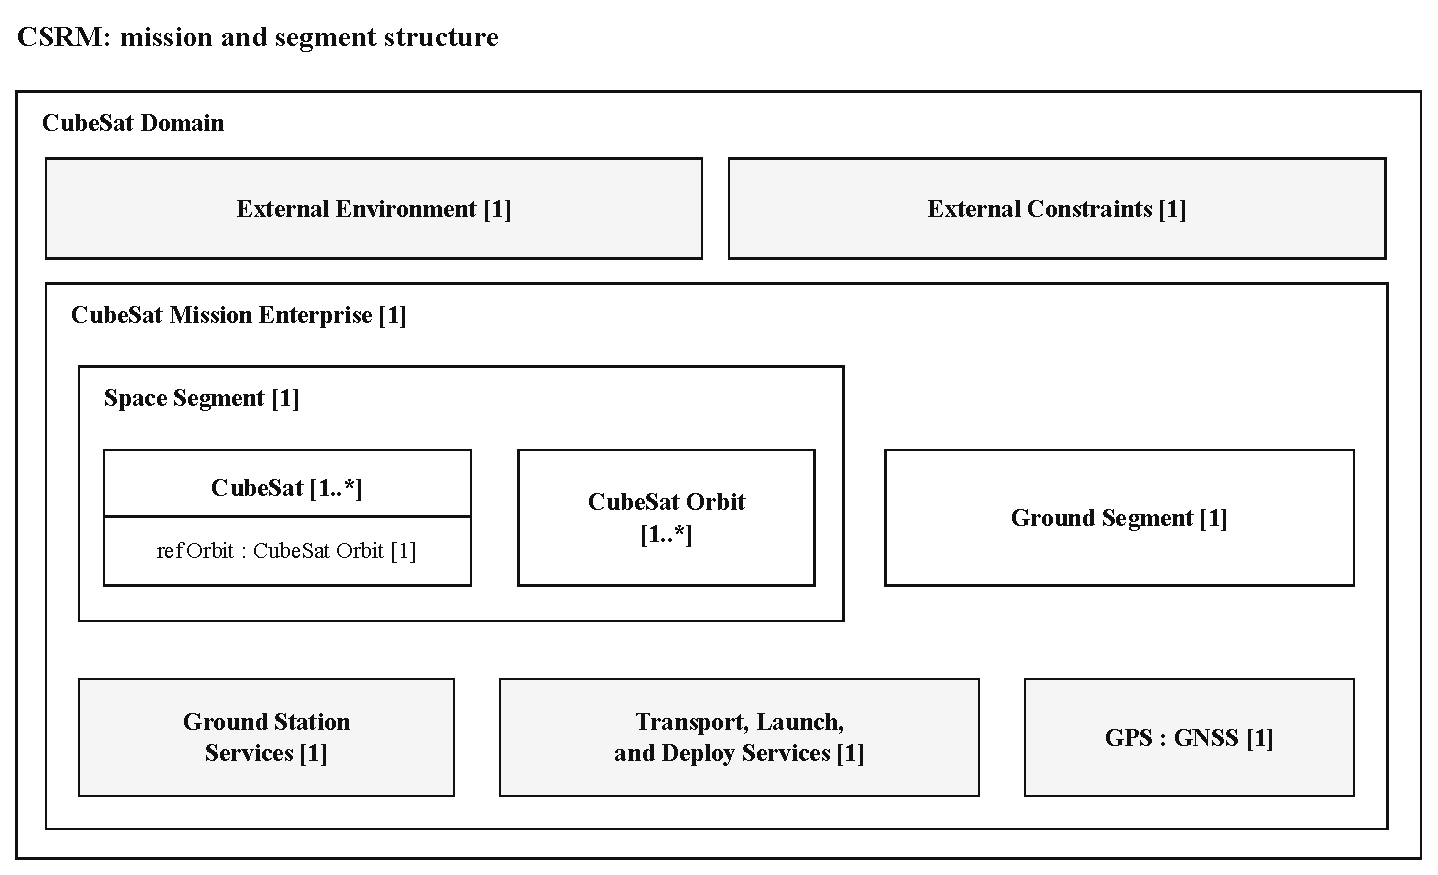
\includegraphics[width=\linewidth,height=\dimexpr\textheight-95pt\relax,keepaspectratio]{fig/csrm-mission-structure.pdf}
\caption[CSRM mission and segment structure.]{CSRM mission and segment structure. Nested rectangles denote composition. Brackets give part multiplicities. Light gray identifies external context and services. Orbits are modeled elements of the Space Segment. Each CubeSat has an orbit reference, with no individual spacecraft-to-orbit pairing specified in this view. Adapted from the CSRM reference model, copyright 2022 INCOSE Space Systems Working Group and OMG Space Domain Task Force, \href{https://creativecommons.org/licenses/by/4.0/}{CC BY 4.0} \citep{incose2025csrmmodel}.}
\label{fig:csrm-mission-structure}
\end{figure}
\clearpage

\begin{figure}[p]
\centering
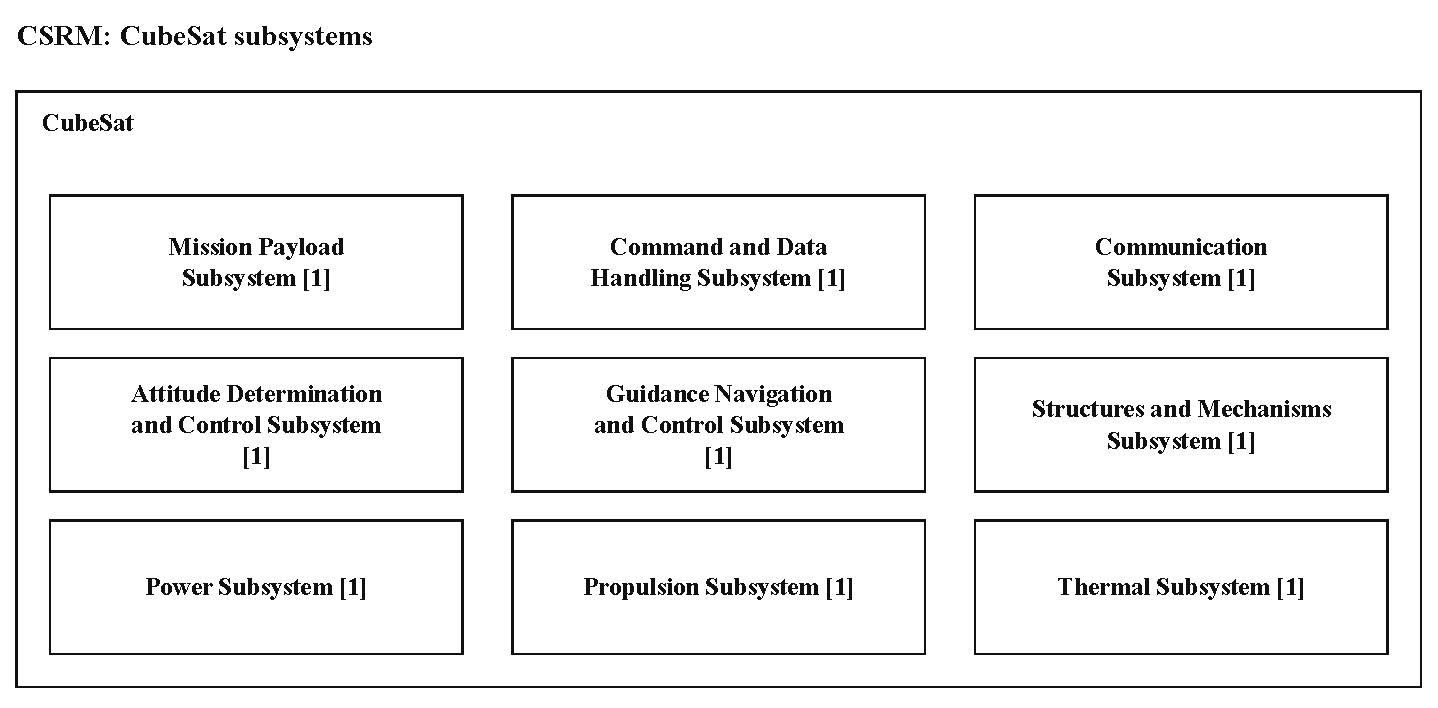
\includegraphics[width=\linewidth,height=\dimexpr\textheight-80pt\relax,keepaspectratio]{fig/csrm-cubesat-subsystems.pdf}
\caption[CSRM CubeSat subsystems.]{CSRM CubeSat subsystems. The reference architecture contains one part for each of nine subsystem categories. Power Subsystem is the EPS. Mission-specific models can omit, combine or refine categories to meet mission needs \citep{kaslow2020csrm}. The view shows logical composition. It specifies no subsystem interfaces or allocation to circuit boards. Adapted from the CSRM reference model \citep{incose2025csrmmodel}.}
\label{fig:csrm-cubesat-subsystems}
\end{figure}
\clearpage

\begin{figure}[p]
\centering
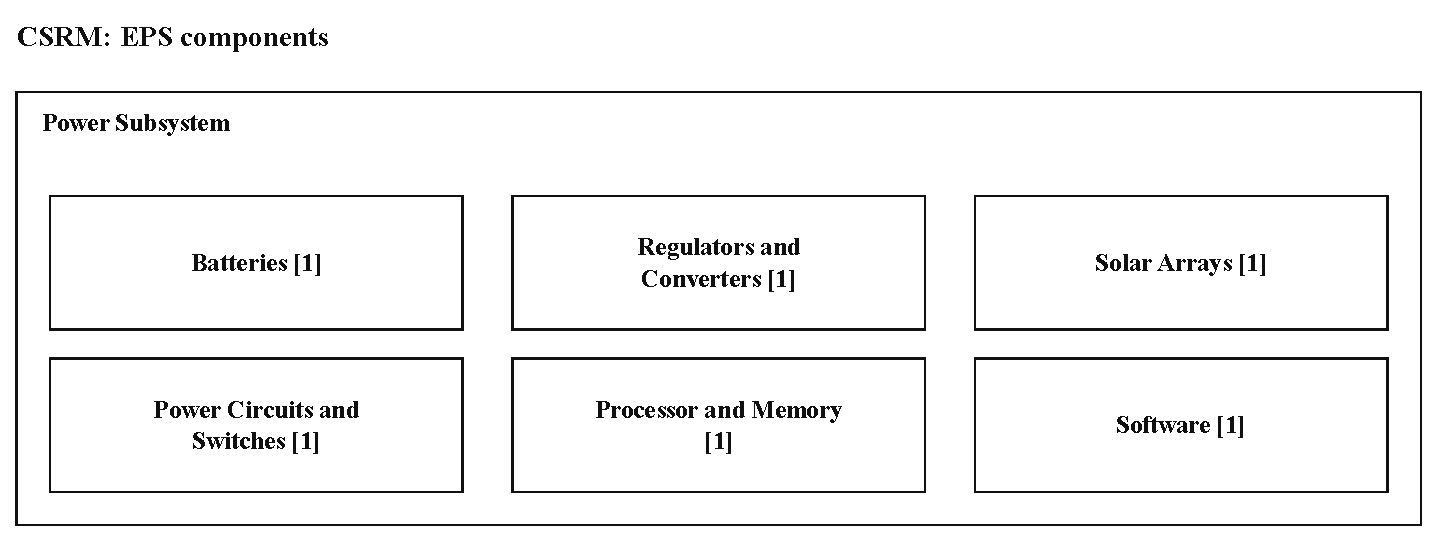
\includegraphics[width=\linewidth,height=\dimexpr\textheight-80pt\relax,keepaspectratio]{fig/csrm-eps-components.pdf}
\caption[CSRM EPS component groups.]{CSRM EPS component groups. The Power Subsystem contains six reference component categories, including processing and software. Batteries and Solar Arrays each denote an aggregate category. Multiplicity [1] identifies one reference part per category. Detailed design will define the numbers of cells, panels, converters and switches, together with their electrical connections. Adapted from the CSRM reference model \citep{incose2025csrmmodel}.}
\label{fig:csrm-eps-components}
\end{figure}
\clearpage
\begin{figure}[p]
\centering
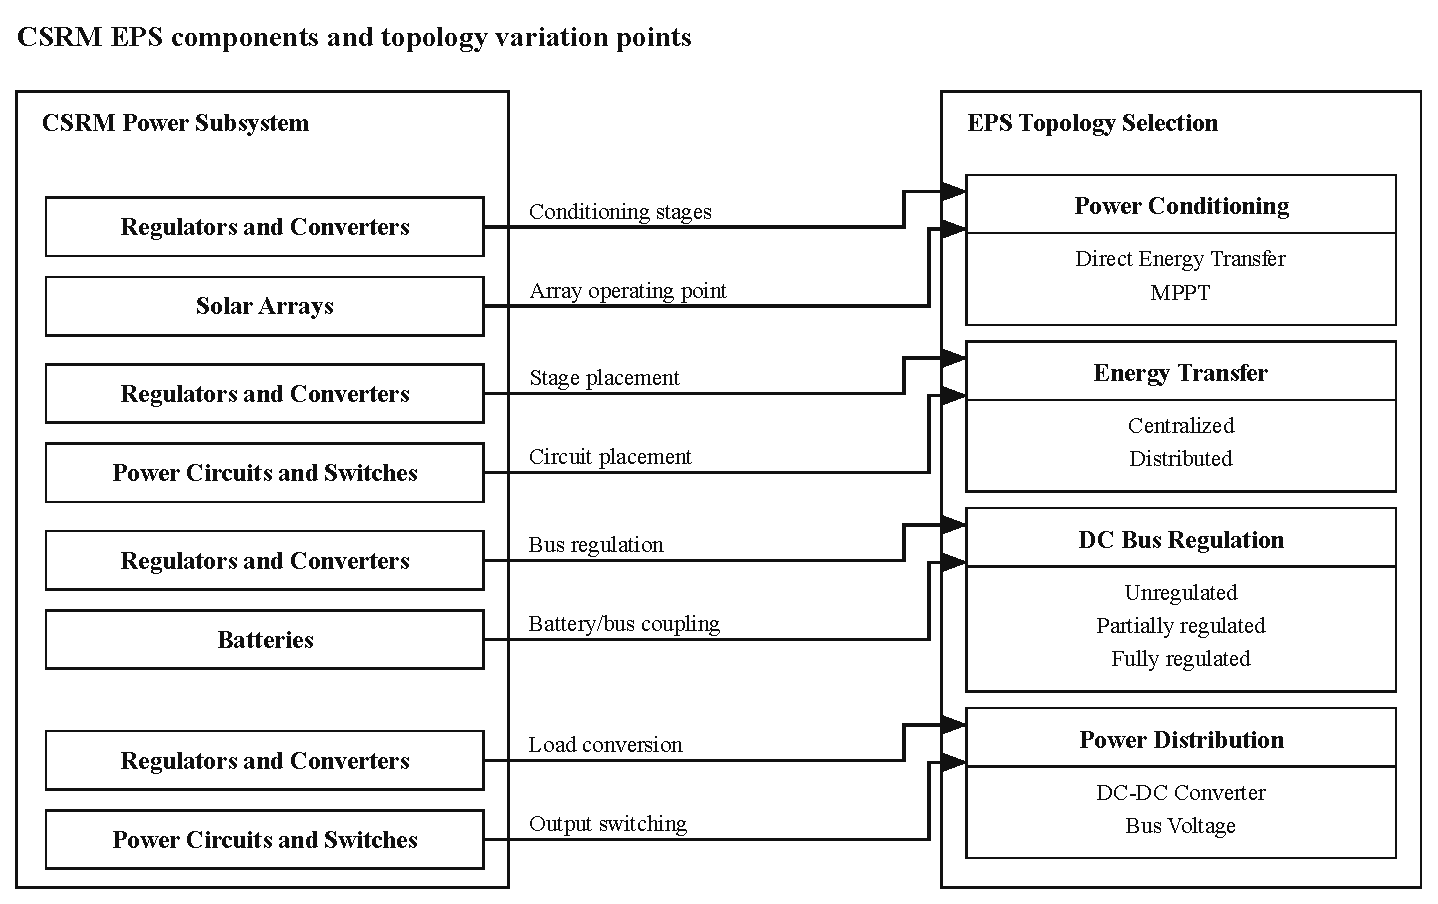
\includegraphics[width=\linewidth,height=\dimexpr\textheight-95pt\relax,keepaspectratio]{fig/csrm-eps-topology.pdf}
\caption[CSRM EPS components and topology variation points.]{CSRM EPS components and topology variation points. Arrows express design associations proposed for this framework. Route labels identify the affected design roles. Repeated component names denote the same CSRM groups \citep{incose2025csrmmodel}. The alternatives follow El Hachimi et al. \citep[Fig.~1, Sec.~4]{handpicked-0003}. The view focuses on hardware topology. Processing and software remain in the reference structure shown in Figure~\ref{fig:csrm-eps-components}. No topology alternative is selected in this view.}
\label{fig:csrm-eps-topology}
\end{figure}
\clearpage
\end{landscape}


\section{Orbit Requirements and Power Budget}

\subsection{Mission analogues from operational descriptions}

When orbit information is unavailable, the framework will accept a plain text concept of operations. It will encode that text and revisioned descriptions of existing missions as semantic embeddings (numerical text vectors), then rank analogues by cosine similarity. Each result will identify the exact mission, source revision and parameter epoch. It will present sourced altitude values or ranges, orbit context and missing fields, while distinguishing flown conditions from intended or study assumptions. Similarity will provide retrieval ranks rather than suitability probabilities. An engineer will review alternatives and explicitly accept each parameter transferred into the mission model. Acceptance will create a mission revision and invalidate dependent results through the normal dependency process. Independent analysis will assess launch opportunities, coverage, revisit, resolution, illumination and orbital constraints. A mission description will establish no unique orbit or validation of its feasibility.

\subsection{Preliminary EPS sizing}

Preliminary EPS sizing will follow El Hachimi et al. \citep[Secs.~2--3, Eqs.~(1)--(10)]{handpicked-0003}.

With altitude $h$ in km, Earth radius $R_e=6378~\mathrm{km}$ and gravitational parameter $\mu=398601~\mathrm{km^3/s^2}$, the orbit, sunlight and eclipse periods (s) are:
\begin{align}
    T_o &= 2\pi\sqrt{\frac{(R_e+h)^3}{\mu}},
    \label{eq:orbit-period} \\
    T_s &= \left(\frac{1}{2}+\frac{\psi}{\pi}\right)T_o,
    \label{eq:sunlight-period} \\
    T_e &= \left(\frac{1}{2}-\frac{\psi}{\pi}\right)T_o,
    \label{eq:eclipse-period} \\
    \psi &= \arccos\left(\frac{R_e}{R_e+h}\right).
    \label{eq:eclipse-geometry}
\end{align}

Subsystem powers and duty cycles give the sunlight and eclipse energies $E_s$ and $E_e$. With corresponding energy path efficiencies $X_s$ and $X_e$, the minimum solar panel power is:
\begin{equation}
    P_{\mathrm{sp}_{\min}} = \frac{\frac{E_s}{X_s}+\frac{E_e}{X_e}}{T_s}.
    \label{eq:minimum-panel-power}
\end{equation}

Solar cell power at end of life (subscript EOL) uses maximum power point voltage $V_{\mathrm{mp}_{\mathrm{EOL}}}$ and current $I_{\mathrm{mp}_{\mathrm{EOL}}}$. The required cell count is $N_{\mathrm{sc}}$:
\begin{align}
    P_{\mathrm{sc}_{\mathrm{EOL}}} &= V_{\mathrm{mp}_{\mathrm{EOL}}} I_{\mathrm{mp}_{\mathrm{EOL}}},
    \label{eq:solar-cell-eol-power} \\
    N_{\mathrm{sc}} &= \frac{P_{\mathrm{sp}_{\min}}}{P_{\mathrm{sc}_{\mathrm{EOL}}}}.
    \label{eq:solar-cell-count}
\end{align}

For mission lifetime $N_{\mathrm{lifetime}}$ in years, $N_{\mathrm{day/year}}$ days per year and $N_{\mathrm{orbit/day}}$ orbits per day, the required cycle count sets the depth of discharge limit $\mathrm{DoD}$. Battery energy includes degradation margin $M$:
\begin{align}
    N_{\mathrm{cycle}} &= N_{\mathrm{lifetime}}\cdot N_{\mathrm{day/year}}\cdot N_{\mathrm{orbit/day}},
    \label{eq:battery-mission-cycles} \\
    N_{\mathrm{cycle}} &= a\cdot \mathrm{DoD}^{b},
    \label{eq:battery-cycle-life} \\
    E_{\mathrm{Battery}} &= \frac{E_e}{\mathrm{DoD}}(1+M).
    \label{eq:battery-energy}
\end{align}

\section{EPS Components and Loads Generic Models}
\label{section:eps-generic-models}

The framework will define reusable models for the six CSRM EPS component groups and for the loads they supply. These models will provide the schema for browsing COTS products and assembling candidate EPS configurations. A catalog entry will describe a particular product and revision. A part usage in a candidate architecture will reference that entry and specify its quantity, supported configuration, installation and connections. One integrated EPS board can implement several CSRM groups. Logical role allocations will reference the same physical usage. Its physical properties will be accounted for once.

\paragraph{Common characterization.}
Luccisano et al. contribute shared component identity, manufacturer, mass, power by operating mode and margins. Their distinction between aggregate and detailed component budgets supports explicit accounting boundaries \citep[Secs.~3.1--3.2]{luccisano2024formalization}. Ceglarek and Bertrand contribute a catalog built from manufacturer datasheets with controlled parameter meanings and units. Their experience with inconsistent datasheets motivates retaining the original value and its reviewed interpretation \citep[Sec.~3]{review-0257}. The proposed schema will extend these contributions with source revisions, operating conditions, uncertainty, supported configurations and interface descriptions. These extensions will make catalog comparisons assessable.

\paragraph{Solar arrays and batteries.}
El Hachimi et al. supply the solar maximum power point and EOL properties, battery energy and cycle-life criteria, and examples of named cells and their arrangements \citep[Secs.~3 and~6.2]{handpicked-0003}. Casado et al. contribute solar current--voltage curves with irradiance and temperature conditions, battery discharge curves and internal resistance \citep[Secs.~2.1 and~2.3]{review-0573}. Boan contributes the series/parallel configuration and mission illumination needed to assess a selected assembly \citep[Sec.~3]{review-0289}. These sources motivate separate cell and assembly records, conditional electrical characteristics and installation geometry. Wijaya et al. contribute fixed commercial product properties alongside sized alternatives. Purchased panels and packs will retain their specified dimensions, mass and ratings \citep[Sec.~III.A--B, Appendix]{review-0145}.

\paragraph{Regulators, converters, power circuits and switches.}
El Hachimi et al. contribute conditioning and bus alternatives, converter input compatibility, independently controlled outputs, protection thresholds, timing and autonomous protection functions \citep[Secs.~4 and~7.1--7.6]{handpicked-0003}. Casado et al. contribute regulator operating modes and transitions, protected output rails, and distribution efficiency estimates based on measurements \citep[Secs.~2.2 and~2.4]{review-0573}. The models will therefore distinguish conversion capabilities, electrical operating limits, loss data, channel organization and protection behavior. A controller integrated circuit record will retain its required external circuit. Its ratings alone will establish no complete converter or protected output.

\paragraph{Processor, memory and software.}
El Hachimi et al. contribute the EPS processor and memory roles, telemetry, output control and hardware/software protection responsibilities \citep[Secs.~7.2--7.5]{handpicked-0003}. Halvorson and Thomas distinguish architecture and interface definitions from implemented behavior and software build dependencies \citep[Secs.~3--4]{review-0853}. The framework will extend these contributions with host compatibility, memory requirements, task timing and versioned service definitions. Software will reference its execution host. Its execution power and physical mass will be included in that host's accounting boundary.

\paragraph{Loads.}
Luccisano et al. contribute power states and their allocation to operating modes \citep[Secs.~3.1--3.2]{luccisano2024formalization}. Casado et al. contribute electrical load profiles and their supply through regulated and unregulated lines \citep[Sec.~2.4]{review-0573}. El Hachimi et al. add maximum-load and protection cases \citep[Secs.~7.4--7.5 and~8.1.4]{handpicked-0003}. The generic load model will combine mode consumption, voltage tolerance, startup pulses, scheduling and shedding constraints. The same description will apply to spacecraft loads and to EPS consumers such as processors and battery heaters.

Figure~\ref{fig:eps-component-models} summarizes the proposed definitions. SysML v2 part definitions will describe hardware and software categories. Attribute definitions will describe structured specifications and physical quantities. Port definitions will describe connection points, and interface definitions will constrain compatible connections \citep[Secs.~7.7, 7.11--7.14 and~9.8]{omg2026sysml2}. Directed command and telemetry items will use requester/provider port conjugation. Physical electrical interfaces will use across voltage and through current quantities with a declared sign convention. Tables~\ref{tab:eps-catalog-records}--\ref{tab:eps-specialized-properties} define the schema summarized in the figure. These definitions are a proposed enrichment of the adopted CSRM structure. In the diagram, each port rectangle carries its reusable type identifier. Multiplicities describe declared connection points, with zero permitting an absent feature. The diagram selects no products or wiring.

\begin{landscape}
\begin{figure}[p]
\centering
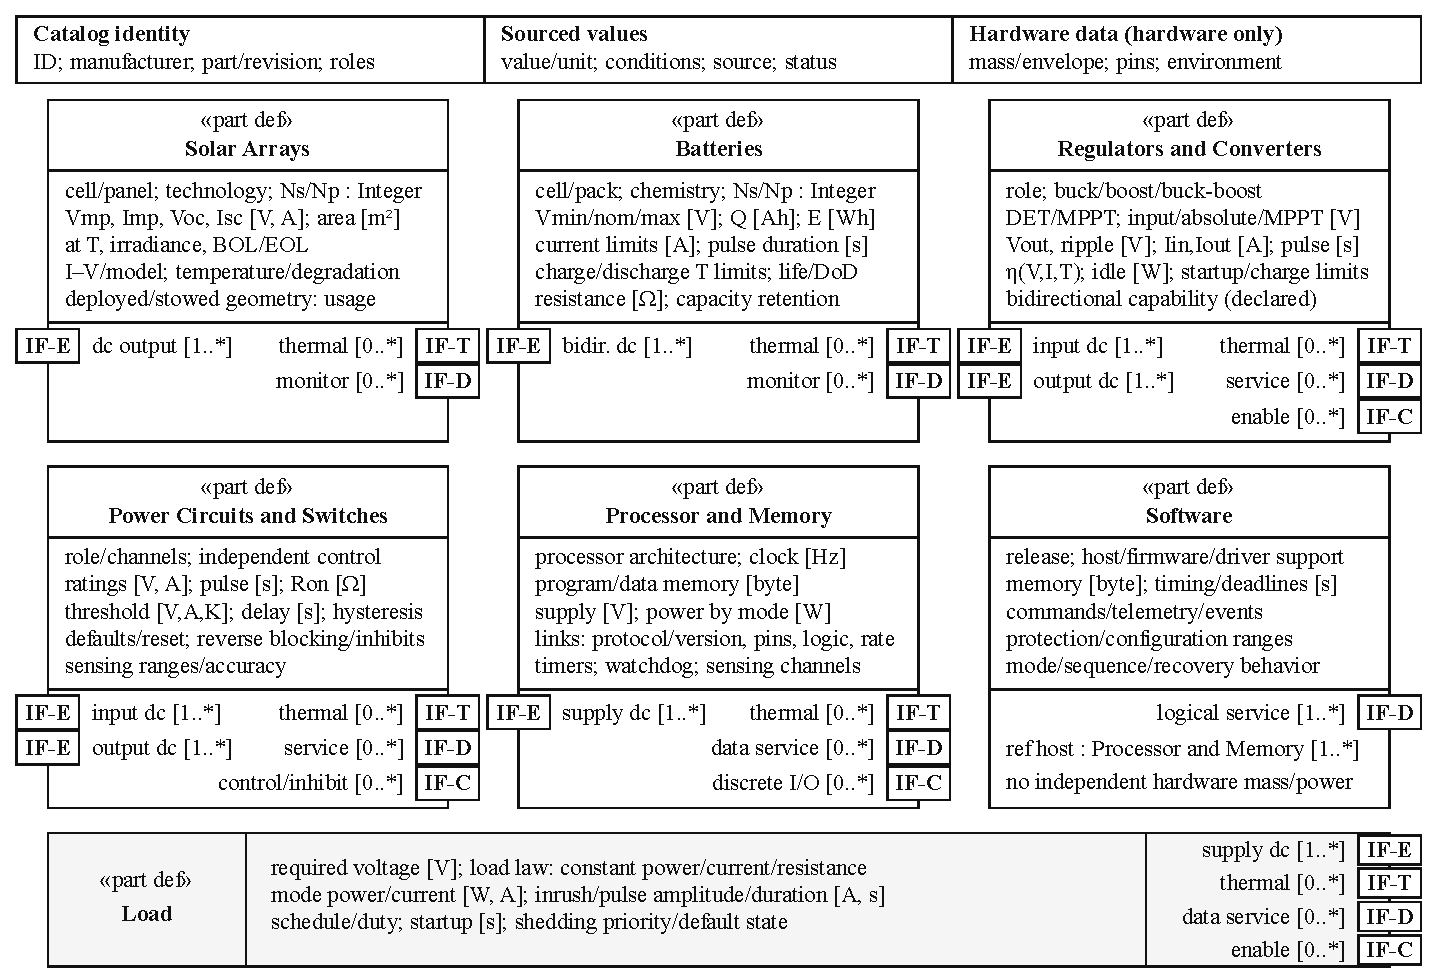
\includegraphics[width=\linewidth,height=\dimexpr\textheight-40pt\relax,keepaspectratio]{fig/eps-component-models.pdf}
\caption[Generic EPS component and load definitions.]{Proposed EPS component and load definitions. Tables~\ref{tab:eps-catalog-records}--\ref{tab:eps-specialized-properties} specify the shared records, port types and properties. Gray identifies external loads.}
\label{fig:eps-component-models}
\end{figure}
\clearpage
\end{landscape}

\subsection{Catalog records and configured part usages}
\label{subsection:eps-catalog-records}

A generic attribute definition will group each structured record in Table~\ref{tab:eps-catalog-records}. Text, Boolean values, enumerations, integers and quantity values will retain their types. Numerical specifications can be scalars, intervals, curves or tables. Quantity values will retain their original units and a consistent internal representation using the SysML v2 quantities and units library. Energy in Wh and charge in Ah will be convertible to J and C. Temperature values will retain their scale. Counts will be integers and efficiencies and duty fractions will be dimensionless.

Every specification will distinguish minimum, typical, maximum, measured and estimated values. Its conditions will identify applicable temperature, irradiance, lifetime, radiation exposure, state of charge, load and pulse duration. A model reference will identify its parameters, validity domain and supported effects. The status of a field will be available, missing or not applicable, with rationale for the latter two. Each required property will have one specification record. An absent value will retain its missing or not-applicable status. Curves and tables will identify independent variables, dependent quantities and interpolation domains. Optional model data will support progressively richer assessments. Missing data will remain visible in catalog browsing and in the scope of any resulting assessment.

{\small
\setlength{\tabcolsep}{4pt}
\renewcommand{\arraystretch}{1.08}
\begin{longtable}{@{}>{\raggedright\arraybackslash}p{0.22\linewidth}>{\raggedright\arraybackslash}p{\dimexpr0.78\linewidth-2\tabcolsep\relax}@{}}
\caption{Shared catalog and configuration records.}\label{tab:eps-catalog-records}\\
\toprule
\textbf{Record} & \textbf{Fields and meaning} \\
\midrule
\endfirsthead
\toprule
\textbf{Record} & \textbf{Fields and meaning} \\
\midrule
\endhead
\bottomrule
\endfoot
Catalog entry & Record identifier and revision, manufacturer, part number, variant, product revision, product level (cell, component, assembly, board or software), provided functions and CSRM roles, included components, supported configurations and compatible accessories. Procurement fields contain supplier, dated price, currency, availability, lead time and lifecycle status. Software entries also identify release, license and supported host/driver versions. \\
Sourced specification & Property identifier, typed value or bound/table, unit and original representation, value meaning, reference conditions, source document/revision/location, observation or retrieval date, uncertainty and review disposition. A numerical model additionally identifies its equations or curves, parameter set and validity domain. \\
Hardware properties & Mass (kg), envelope dimensions (m), keep-out and mounting geometry, connector and terminal pin maps, operating/storage temperature limits (K), thermal contacts and applicable thermal model. Qualification and radiation records identify tested article/revision, conditions, exposure, outcomes and evidence. Flight heritage is recorded with its configuration and environment. \\
Accounting boundary & For each mass, volume, price or consumption specification, identify whether it covers the complete product or named internal components. Record included consumers and losses. Assemblies retain their own identity and references to their contents. Software physical resources belong to its host. \\
Configured usage & Unique installed-part identity, catalog-entry revision, quantity, supported configuration and settings, location/orientation, deployment state, selected ports and function/requirement allocations. Array placement includes active face normals, usable area and packing fraction. Load and software assignments identify their supplying channel and execution host, respectively. \\
Connection & Endpoint identities and physical terminal/return mapping, harness or adapter identity, resistance (\(\Omega\)) and current rating (A) under stated conditions. Data connections add protocol/version, endpoint roles, signal levels, rate (bit/s), addressing and timing. Discrete lines add polarity, default/fault state and inhibit logic. Each physical auxiliary item has its own usage or an identified assembly accounting boundary. \\
Mission scenario & Orbit and attitude history, illumination, temperatures or thermal boundary conditions, lifetime case, load modes and schedules, allowed transitions, initial battery state, discharge/reserve criteria, assessment duration and energy-closure tolerance (J). Allocations identify mass, volume, installation envelope, cost and required service behavior. Each scenario and criterion retains its source and revision. Assessment scope identifies lifecycle phase, intended use, required evidence and accepted modeling assumptions. \\
\end{longtable}
}

Catalog definitions will separate supported configurations from installed choices. A finished panel or battery pack will retain its fixed internal arrangement. A configurable product will expose only the arrangements supported by its supplier. An assembly built from catalog cells will identify the cells and additional protection, interconnects and packaging. Its resulting characteristics will be derived at the assembly level. Individual component records will remain browseable alongside complete EPS boards.

\subsection{Reusable interface definitions}
\label{subsection:eps-port-types}

Table~\ref{tab:eps-port-types} specifies four reusable interface types. Separate SysML v2 port and interface definitions will specify each entry's endpoints and connection constraints. Their identifiers are local to the EPS design model and distinct from the framework interfaces in Chapter~\ref{ch:solucion}. Each interface usage will connect declared port usages. Physical endpoint descriptions will retain the connector, pin and return mapping. A software service will bind to its host's physical endpoint. A product can provide no data interface, as with a passive cell. Port multiplicities will be resolved for the selected product and configuration.

{\small
\setlength{\tabcolsep}{4pt}
\renewcommand{\arraystretch}{1.08}
\begin{longtable}{@{}>{\raggedright\arraybackslash}p{0.22\linewidth}>{\raggedright\arraybackslash}p{\dimexpr0.78\linewidth-2\tabcolsep\relax}@{}}
\caption{EPS port and interface types.}\label{tab:eps-port-types}\\
\toprule
\textbf{Type} & \textbf{Port features and interface meaning} \\
\midrule
\endfirsthead
\toprule
\textbf{Type} & \textbf{Port features and interface meaning} \\
\midrule
\endhead
\bottomrule
\endfoot
IF-E: electrical & A DC terminal pair has voltage \(v\) (V) relative to its declared return, current \(i\) (A) positive into its owner, source/sink/bidirectional capability, and operating and absolute limits. An ideal interface relates across voltages and through currents. Harnesses, switches, converters and isolating devices retain their own voltage drops and return relationships. \\
IF-T: thermal & A thermal boundary has temperature \(T\) (K), heat flow \(\dot Q\) (W) positive into its owner, and contact/boundary identity. Thermal contacts and models specify resistance or conductance and applicable boundary conditions. The catalog records supported thermal contacts separately from mission temperatures. \\
IF-D: data service & A provider receives Command and Configuration items and emits Telemetry and Event items. A requester uses the conjugated directions. Item definitions contain identifier, target/channel, payload types, quantities/units, permitted ranges, time/validity meaning and applicable sampling, response or deadline criteria. Hardware transport records contain protocol/version, pin mapping, electrical levels, rate, endpoint roles and address. Software refers to that transport through its host. \\
IF-C: discrete control & A directed control, enable or inhibit signal has logical meaning, electrical input/output limits, polarity, pin/return mapping, default and fault state, response time and applicable inhibit truth table. Hardware protection and flight inhibits retain their authority and autonomy from software commands. \\
\end{longtable}
}

\subsection{Component and load properties}
\label{subsection:eps-specialized-properties}

Table~\ref{tab:eps-specialized-properties} gives the specialized attributes and port usages. Product levels, chemistries, topologies, modes, load laws and reset policies will use enumerations. Counts and memory sizes will use integers. Capabilities will use Boolean values or sets of named options. Versions and document identifiers will use text. Configurations, channels, tasks and geometry will use structured records or collections with declared multiplicities. Every numerical characteristic uses the record for sourced specifications. Temperature and lifetime dependence can be represented by bounded tables or applicable models. A property used for preliminary sizing can therefore be replaced by richer characterized data while preserving its quantity, source and interface meaning.

{\small
\setlength{\tabcolsep}{4pt}
\renewcommand{\arraystretch}{1.08}
\begin{longtable}{@{}>{\raggedright\arraybackslash}p{0.22\linewidth}>{\raggedright\arraybackslash}p{\dimexpr0.78\linewidth-2\tabcolsep\relax}@{}}
\caption{Specialized EPS component and load definitions.}\label{tab:eps-specialized-properties}\\
\toprule
\textbf{Definition} & \textbf{Attributes and port usages} \\
\midrule
\endfirsthead
\toprule
\textbf{Definition} & \textbf{Attributes and port usages} \\
\midrule
\endhead
\bottomrule
\endfoot
Solar Arrays & Product level, cell technology, supported series/parallel counts \(N_s,N_p\), active area \(A\) (m\(^{2}\)), \(V_{\mathrm{mp}},V_{\mathrm{oc}}\) (V), \(I_{\mathrm{mp}},I_{\mathrm{sc}}\) (A), current--voltage/model data and temperature/degradation characteristics at identified beginning/end-of-life conditions. Panel definitions identify independent sections, bypass/reverse-blocking features and supported deployment states. Installed orientation and packing belong to the usage. Ports: DC output IF-E [1..*], thermal IF-T [0..*] and monitoring IF-D [0..*]. \\
Batteries & Product level, chemistry, supported \(N_s,N_p\), minimum/nominal/maximum voltage (V), rated charge \(Q\) (C, commonly Ah), rated energy \(E\) (J, commonly Wh), charge/discharge current limits (A) with pulse durations (s), separate charging/discharging temperature limits, cycle-life versus DoD data, retained-energy/charge factors \(f_E,f_Q\), energy efficiencies \(\eta_c,\eta_d\), coulombic efficiencies \(\eta_{Q,c},\eta_{Q,d}\), internal resistance (\(\Omega\)) and voltage/discharge model. Pack features identify balancing, protection, sensing and heaters included in the product. Ports: bidirectional DC IF-E [1..*], thermal IF-T [0..*] and monitoring IF-D [0..*]. \\
Regulators and Converters & Conversion/charging roles, buck/boost/buck--boost/linear or direct-transfer implementation, DET/MPPT capabilities, input operating interval and absolute limit (V), tracking interval (V), permissible source current (A), output voltage/ripple (V), continuous/pulse input and output limits (A, s), startup conditions and conversion envelope \(\mathcal C\). Loss or efficiency maps \(P_{\mathrm{loss}}\), \(\eta\) identify voltage, current, temperature, mode and whether idle power \(P_0\) (W) is included. Charger data identify chemistry, supported cell counts, voltage/current limits, termination and temperature rules. Ports: DC input and output IF-E [1..*] each, with reverse transfer explicitly declared, thermal IF-T [0..*], service IF-D [0..*] and enable IF-C [0..*]. \\
Power Circuits and Switches & Circuit role, channel count and independently controlled/protected groups, default states, voltage and continuous/pulse current ratings (V, A, s), on resistance (\(\Omega\)), idle power (W), sensing ranges/accuracy, reverse-current blocking and supported inhibits. Protection data contain threshold bounds (V, A, K), trip-time curves (s), hysteresis, safe operating area, reset/retry policy and hardware/software responsibility. The usage sets values within these supported ranges. Ports: DC input and output IF-E [1..*] each, thermal IF-T [0..*], service IF-D [0..*] and control/inhibit IF-C [0..*]. Harness records use the applicable circuit and connection properties. \\
Processor and Memory & Processor architecture, clock rate (Hz), available program/data memory (byte), supply interval (V), consumption by mode (W), physical link definitions, timers, watchdog and sensing/input/output channel capabilities. Resource availability identifies reservations by supplied firmware. Ports: supply IF-E [1..*], thermal IF-T [0..*], service IF-D [0..*] and discrete input/output IF-C [0..*]. \\
Software & Release, compatible host/firmware/driver versions, required program/data memory (byte), task periods, execution bounds and deadlines (s) for the declared host, supported commands/telemetry/events, parameter ranges, mode transitions, sequencing, shedding and recovery behavior. A reference identifies execution hosts of type Processor and Memory [1..*] and task/resource allocations. Logical service ports are IF-D [1..*]. Physical mass, electrical consumption and thermal dissipation are assigned to the host. \\
Load & Required supply interval (V), load law (constant power, constant current, resistance or characterized curve), \(P_{\ell m}\) (W), \(I_{\ell m}\) (A) or \(R_{\ell m}\) (\(\Omega\)) by mode \(m\), startup/pulse amplitude and duration (A, s), startup time (s), schedule/duty fraction, default state, shedding priority and essential-service constraints. Heat dissipation or a thermal model identifies the thermal load. Startup/pulse intervals identify whether they replace or supplement steady consumption. Ports: supply IF-E [1..*], thermal IF-T [0..*], service IF-D [0..*] and enable IF-C [0..*]. \\
\end{longtable}
}

\section{EPS Component Selection}
\label{section:eps-component-selection}

Selection will operate on the definitions in Section~\ref{section:eps-generic-models}. Jacobs and Selva provide forward evaluation of selected products and backward enumeration of catalog combinations, with critical requirements filtering the feasible set before cost comparison \citep[Sec.~2]{citation-1136}. Wijaya et al. contribute architecture choices and dependencies followed by numerical evaluation \citep[Secs.~4.1--4.4]{review-0055}. Their COTS study distinguishes fixed purchased properties from continuously sized components \citep[Sec.~III]{review-0145}. GREATCUBE+ contributes repeated compatibility assessment after component replacement \citep[Secs.~2.2.1--2.2.2]{review-0711}. Boan contributes the electrical configuration and mission energy-balance iteration \citep[Secs.~3--4]{review-0289}. The following equations and algorithm synthesize these contributions for the proposed schema. Applicable criteria and evidence levels will follow the declared lifecycle phase and intended use. Preliminary electrical feasibility and component qualification will retain distinct assessment scopes.

\subsection{Catalog browsing and architecture alternatives}

Browsing will support filters for CSRM role, product level, manufacturer, supported topology, electrical ranges, environmental conditions, physical envelope, interfaces and procurement constraints. Results will expose the source and conditions of each compared value. Unknown properties will be shown separately from known violations. A typical rating will establish no guaranteed limit unless an engineer accepts a sourced conservative bound. Datasheet maxima, operating limits and measured performance will retain their distinct meanings.

A candidate \(d\) will comprise topology choices, catalog revisions, integer quantities, supported configurations, connections, assignments of loads to channels and allocations of software to hosts. Topology choices will follow Figure~\ref{fig:csrm-eps-topology}: DET or MPPT conditioning, centralized or distributed transfer, bus regulation, and direct or converted supply for each output rail. Direct and converted outputs can coexist. Product capabilities and dependencies will restrict these combinations. Required functions, external controller circuitry and auxiliaries must be covered by identified installed usages. Logical role coverage alone will establish no current capacity, fault independence or geometric fit.

Finished product properties will remain fixed during selection. Series/parallel changes will be permitted for configurable products and assemblies of catalog cells. Supplier configurations or engineer-declared assembly bounds will keep the enumeration finite. A product substitution will trigger renewed sizing, loss, interface and scenario assessments. New conditions or load schedules will remain explicit scenario revisions.

\subsection{Generation and storage configuration}

Equations~\eqref{eq:minimum-panel-power}--\eqref{eq:battery-energy} will provide preliminary screens for each candidate. The solar cell count will be recalculated from the selected cell's EOL data and rounded upward for physical assembly. For identical cells distributed over sections \(g\), the installed count will satisfy the preliminary lower bound
\begin{equation}
    \sum_g N_{s,g}^{\mathrm{pv}}N_{p,g}^{\mathrm{pv}}\geq\left\lceil N_{\mathrm{sc}}\right\rceil,
    \qquad N_{s,g}^{\mathrm{pv}},N_{p,g}^{\mathrm{pv}}\in\mathbb Z_{>0}.
    \label{eq:pv-integer-configuration}
\end{equation}
Sections on differently illuminated faces will be evaluated separately. Installed cell count will be followed by an illumination-dependent generation assessment. With irradiance, temperature and orientation from scenario \(\sigma\), the selected current--voltage model and operating point give each section's available source power \(P_{g,\mathrm{avail}}(t,\sigma)\). At the same source boundary as Equation~\eqref{eq:minimum-panel-power}, a screen using average power during sunlight is
\begin{equation}
    \frac{1}{T_s}\int_{\mathrm{sunlight}}\sum_g P_{g,\mathrm{avail}}(t,\sigma)\,dt
    \geq P_{\mathrm{sp}_{\min}}.
    \label{eq:array-generation-screen}
\end{equation}
This screen will use the candidate's attainable operating point under DET or MPPT and its applicable path efficiencies \(X_s,X_e\). Stored energy, charge acceptance and load peaks will be assessed separately below.

For a matched section connected to MPPT input \(r\), the following conservative checks will use extrema over the applicable temperature, irradiance and lifetime conditions:
\begin{align}
    [N_s^{\mathrm{pv}}V_{\mathrm{mp}}^{\mathrm{lo}},
     N_s^{\mathrm{pv}}V_{\mathrm{mp}}^{\mathrm{hi}}]
    &\subseteq[V_{\mathrm{track},r}^{\mathrm{lo}},V_{\mathrm{track},r}^{\mathrm{hi}}],
    \label{eq:mppt-voltage-compatibility}\\
    N_s^{\mathrm{pv}}V_{\mathrm{oc}}^{\mathrm{hi}}&\leq V_{\mathrm{abs},r},
    \qquad N_p^{\mathrm{pv}}I_{\mathrm{sc}}^{\mathrm{hi}}\leq I_{\mathrm{source,allow},r}.
    \label{eq:pv-input-ratings}
\end{align}
Here \(V_{\mathrm{abs},r}\) is the absolute input limit and \(I_{\mathrm{source,allow},r}\) is the permissible source current from the converter specification. Startup and operating-voltage limits will also be checked. Shared trackers will require a compatible combined current--voltage characteristic. DET configurations will instead use the array characteristic at the battery/bus operating voltage, including blocking and wiring drops.

For an assembly of identical battery cells, the initial estimates will be
\begin{equation}
    \begin{aligned}
        E_{\mathrm{pack,BOL}}&=N_s^{\mathrm{bat}}N_p^{\mathrm{bat}}E_{\mathrm{cell,BOL}},\\
        Q_{\mathrm{pack,BOL}}&=N_p^{\mathrm{bat}}Q_{\mathrm{cell,BOL}}.
    \end{aligned}
    \label{eq:battery-assembly-capacity}
\end{equation}
\begin{equation}
    \begin{aligned}
        \relax[V_{\mathrm{pack}}^{\mathrm{lo}},V_{\mathrm{pack}}^{\mathrm{hi}}]
        &=[N_s^{\mathrm{bat}}V_{\mathrm{cell}}^{\mathrm{lo}},N_s^{\mathrm{bat}}V_{\mathrm{cell}}^{\mathrm{hi}}],\\
        I_{\mathrm{pack,allow}}&=N_p^{\mathrm{bat}}I_{\mathrm{cell,allow}}.
    \end{aligned}
    \label{eq:battery-assembly-ratings}
\end{equation}
Current limits will retain separate charging, discharging and pulse conditions. The DoD limit will use the selected cell's cycle-life data under applicable conditions. Coefficients \(a,b\) in Equation~\eqref{eq:battery-cycle-life} will retain their sourced fit domain. Packaging, interconnects, balancing and protection can further restrict these cell-based estimates. A finished pack will use its supplier's pack ratings. The preliminary capacity screen will compare \(E_{\mathrm{pack,BOL}}\) with \(E_{\mathrm{Battery}}\). EOL assessment will use the specified retained capacity or an applicable aging model, with \(E_{\mathrm{pack,EOL}}=f_EE_{\mathrm{pack,BOL}}\) where that factor is valid. Margin \(M\) will be applied once in preliminary sizing. The physical EOL model will use retained capacity without applying \(M\) again. The selected chemistry, cell count, charging voltage/current, temperature restrictions and termination rules will be matched to the charger.

\subsection{Connections, loads and operating limits}

At an ideal IF-E connection, consistent terminal and return mapping will give
\begin{equation}
    v_a=v_b,\qquad i_a+i_b=0.
    \label{eq:electrical-interface-conservation}
\end{equation}
Current is positive into each connected part. A physical path will include its declared losses. For a resistive supply-and-return path,
\begin{equation}
    V_\ell=V_r-I_{\mathrm{path}}R_{\mathrm{path}},
    \label{eq:load-path-drop}
\end{equation}
where \(V_r\) is the supplying rail voltage and \(R_{\mathrm{path}}\) includes the relevant harness, contact and conducting-switch resistance once. Shared paths will carry the sum of their branch currents. Isolation and differing returns will require an explicitly modeled interface or adapter.

The load law in Table~\ref{tab:eps-specialized-properties} will determine current at the actual terminal voltage:
\begin{equation}
    I_\ell(V_\ell,m)=
    \begin{cases}
        P_{\ell m}/V_\ell, & \text{constant power},\\
        I_{\ell m}, & \text{constant current},\\
        V_\ell/R_{\ell m}, & \text{resistive load}.
    \end{cases}
    \label{eq:generic-load-law}
\end{equation}
A characterized load will use its supplied curve or model instead. Mode schedules and pulse records will identify simultaneous demand. For every active load and applicable scenario,
\begin{equation}
    V_\ell^{\mathrm{req,lo}}\leq V_\ell(t,\sigma)\leq V_\ell^{\mathrm{req,hi}},
    \qquad
    \sum_{\ell\in\mathcal L_r}I_\ell(t,\sigma)
    \leq I_{r,\mathrm{allow}}(T,\text{duration}).
    \label{eq:rail-load-compatibility}
\end{equation}
\(\mathcal L_r\) contains loads assigned to rail or channel \(r\). Shared channel groups and converter inputs will be checked against their aggregate ratings. Continuous operation and startup/pulse events will use their respective limits. A converter's operating tuple \((V_{\mathrm{in}},V_{\mathrm{out}},I_{\mathrm{out}},T)\) must lie within its sourced conversion envelope \(\mathcal C_r\). This will include dropout, conversion-ratio and startup restrictions.

Demand will be propagated upstream through the selected paths using
\begin{equation}
    P_{\mathrm{in},r}=P_{\mathrm{out},r}+P_{\mathrm{loss},r}.
    \label{eq:conversion-loss-accounting}
\end{equation}
An efficiency specification implies \(P_{\mathrm{loss},r}=P_{\mathrm{out},r}(\eta_r^{-1}-1)\) within its stated domain. Separate idle power will be added only when excluded from that efficiency. Zero-load and disabled states will use their own consumption data. An aggregate board-input specification and its included internal loads will contribute once. The same rule will prevent software execution from becoming an additional physical load alongside its host.

Protection assessment will compare legitimate steady and pulse demand with the no-trip region, then compare fault interruption with the protected path's current, energy and safe-operating-area limits. Threshold tolerances and interruption times will be evaluated together against the protected path's continuous, pulse and safe-operating-area limits. Pulse tolerance, trip delay, hysteresis, retry and default states will be checked separately. Declared hardware protection and flight inhibits must remain effective under the specified processor/software failure conditions.

Hardware temperatures will remain within the applicable operating intervals. Battery charging and discharging will use their distinct temperature restrictions. Qualification and radiation evidence will be assessed against the mission environment and exact product configuration. An environmental evidence gap will remain an unresolved assessment, with no inferred qualification from flight heritage alone.

IF-D and IF-C checks will compare directed features, quantities, identifiers, pin assignments, logic levels, protocols, versions, address allocation, timing and startup/fault behavior. A common connector shape or protocol name will establish no complete compatibility. Software-host checks will include architecture, supplied firmware and drivers, available memory and execution assumptions. For tasks \(a\) allocated to host \(h\), preliminary resource screens will be
\begin{equation}
    \sum_{a\in\mathcal A_h}B_a^{\mathrm{data}}\leq B_h^{\mathrm{available}},
    \qquad
    \sum_{a\in\mathcal A_h}\frac{C_a}{T_a}\leq U_h^{\mathrm{allocated}},
    \label{eq:software-resource-screen}
\end{equation}
where \(B_a^{\mathrm{data}}\) is required data memory, \(C_a\) is execution time on the declared host, \(T_a\) is task period and \(U_h^{\mathrm{allocated}}\) is the allocated processor utilization. Program storage will be checked similarly. These screens will establish no deadline guarantee. Scheduling and service-response evidence will be assessed against the declared deadlines. Supplied opaque firmware will require applicable vendor or assessment evidence for the claimed services and timing.

\subsection{Mission energy balance and resource budgets}

Surviving configurations will be assessed over the mission scenarios using their selected component models. Solar geometry, temperature, battery voltage, converter operating points and loss maps will remain coupled. At a common reference boundary outside the battery terminals, let \(P_g\) be solar power available after conditioning and \(P_d\) the upstream demand of all loads and distribution paths, including EPS consumption. Both powers will include the applicable external path losses. Battery internal losses will be represented by its efficiencies or selected battery model. The net available power is \(P_\Delta=P_g-P_d\). A preliminary energy model will use
\begin{align}
    P_{\mathrm{dis},k}&=\max(-P_{\Delta,k},0),
    \label{eq:battery-discharge-demand}\\
    P_{\mathrm{ch},k}&=\min\left\{\max(P_{\Delta,k},0),\,
    P_{\mathrm{ch,allow},k},\,
    \frac{E_{\max}-E_k}{\eta_{c,k}\Delta t},\,
    \frac{v_{b,k}(Q_{\max}-Q_k)}{\eta_{Q,c}\Delta t}\right\},
    \label{eq:battery-charge-acceptance}\\
    E_{k+1}&=E_k+\left(\eta_{c,k}P_{\mathrm{ch},k}
    -\frac{P_{\mathrm{dis},k}}{\eta_{d,k}}\right)\Delta t.
    \label{eq:battery-energy-propagation}
\end{align}
Here energy is in J, power in W and \(\Delta t\) in s. \(v_{b,k}\) is battery terminal voltage at step \(k\). \(E_{\max}\) is a conservative fixed energy capacity for the run's temperature/lifetime case. Charge acceptance \(P_{\mathrm{ch,allow}}\) will include battery and charger voltage, current, temperature and termination limits. Unused solar surplus will follow the selected circuit's curtailment or shunt capability. Resulting voltage and heat will be assessed. Required discharge above a battery or path limit will be a failure. Energy shortages will be retained as failures. Assessment will stop at an invalid battery state. Terminal-voltage and transient assessments will use the applicable battery and circuit models.

Charge-based state of charge \(z\) will remain distinct from normalized stored energy. With battery-port current \(i_b\) positive into the battery, a coulomb-counting model will use
\begin{equation}
    \begin{aligned}
        Q_{k+1}&=Q_k+\left(\eta_{Q,c}\max(i_{b,k},0)
        -\frac{\max(-i_{b,k},0)}{\eta_{Q,d}}\right)\Delta t,\\
        z_k&=Q_k/Q_{\max}.
    \end{aligned}
    \label{eq:battery-charge-propagation}
\end{equation}
\(Q\) is remaining charge in C and \(Q_{\max}\) is its applicable retained capacity. Current will be obtained from the battery terminal voltage and charge/discharge power. The energy and charge models will require consistent characterized data, including their respective efficiencies. Full-charge limits will constrain both states. A richer battery model can replace these preliminary balances while retaining the same interface and loss boundaries. An energy-only assessment will leave charge-based DoD and voltage criteria unassessed without an applicable mapping.

For nominal repeating conditions, the criteria will include
\begin{equation}
    z_k\geq1-\mathrm{DoD}_{\max},\qquad
    E_{\mathrm{end}}\geq E_{\mathrm{start}}-\epsilon_E,
    \label{eq:nominal-energy-feasibility}
\end{equation}
with declared initial state and numerical energy-closure tolerance \(\epsilon_E\). Survival and recovery cases will use their own allowed duration, initial state, essential loads and minimum reserve. They will retain any authorized exceptional discharge separately from nominal cycle-life criteria. Load shedding will follow the declared service and priority constraints.

For uniquely accounted physical or procurement usages \(j\), quantity \(q_j\) will give
\begin{equation}
    \begin{aligned}
        m_{\mathrm{EPS}}&=\sum_jq_jm_j\leq m_{\mathrm{allocated}},\\
        V_{\mathrm{occupied}}&=\sum_jq_jV_j\leq V_{\mathrm{allocated}},\\
        C_{\mathrm{EPS}}&=\sum_jq_jc_j+C_{\mathrm{additional}}.
    \end{aligned}
    \label{eq:eps-product-budgets}
\end{equation}
\(m_j,V_j,c_j\) denote product mass, occupied envelope volume and unit price, respectively. The budget will include required harnesses, adapters, packaging and protection. \(C_{\mathrm{additional}}\) will contain separately declared integration, licensing or qualification costs excluded from product prices. Currency conversion will retain its rate and date. Missing prices or effort estimates will limit the cost comparison. Volume totals will be followed by installation-envelope, keep-out, mounting, connector-access and stack-height checks. Aggregate and internal component properties will follow their accounting boundaries independently for each budget.

\subsection{Parametric EPS requirements}
\label{subsection:eps-parametric-requirements}

Table~\ref{tab:eps-parameter-requirements} proposes requirements on the modeled EPS and its service to the loads. They synthesize the cited design methods using the properties in Tables~\ref{tab:eps-catalog-records}--\ref{tab:eps-specialized-properties}. Component and load limits, allocations and supplied scenarios determine the criteria. The requirements apply to the selected functions and configurations across their specified modes, temperatures, illumination, lifetime cases, schedules and pulses. Bounded calculations and supplied histories can support concept assessment through MR-03. Steady, pulse and state bounds suffice where they establish the predicates. More detailed model and software assessments can refine these results in MR-04--06.

A requirement passes when its predicate holds throughout the applicable conditions. A known violation fails. Missing decisive parameters or bounds spanning compliance and violation leave the assessment unassessed. An absent optional function is not applicable. Operating limits and absolute maxima retain their separate meanings. Pulse records determine whether startup demand replaces or supplements steady consumption. The symbol \(z_{\min,\sigma}\) denotes the minimum charge-based state of charge permitted by scenario \(\sigma\), including its applicable discharge and reserve criteria. Energy reserve criteria apply directly to stored energy.

\begingroup
\small
\setlength{\tabcolsep}{4pt}
\setlength{\parskip}{0pt}
\setlength{\LTpre}{0.4\baselineskip}
\setlength{\LTpost}{0.4\baselineskip}
\renewcommand{\arraystretch}{1.06}
\setlength{\ReportTableBodyWidth}{\dimexpr\linewidth-6\tabcolsep\relax}
\begin{longtable}{@{}P{0.09\ReportTableBodyWidth}P{0.37\ReportTableBodyWidth}P{0.29\ReportTableBodyWidth}P{0.25\ReportTableBodyWidth}@{}}
\caption{Parameter-based EPS and load requirements.}\label{tab:eps-parameter-requirements}\\
\toprule
\textbf{ID} & \textbf{Requirement and equation or algorithm} & \textbf{Pass/fail criterion} & \textbf{Rationale} \\
\midrule
\endfirsthead
\toprule
\textbf{ID} & \textbf{Requirement and equation or algorithm} & \textbf{Pass/fail criterion} & \textbf{Rationale} \\
\midrule
\endhead
\bottomrule
\endfoot
\multicolumn{4}{@{}l}{\textbf{Configuration and power paths}} \\*
EPS-01\phantomsection\label{epsreq:EPS-01} & The EPS shall use supported product configurations and settings. Compare each configured usage, including series/parallel counts, with its supported options or declared cell-assembly bounds and required external circuitry. & Every choice is supported. Configured cell counts are positive integers. Required external circuits and adapters are included. Finished panels and packs retain their fixed properties and internal arrangement. & Purchased products constrain realizable configurations \citep[Sec.~III.A--B]{review-0145}. \\
EPS-02\phantomsection\label{epsreq:EPS-02} & The solar arrays shall meet the preliminary generation bound in Equation~\eqref{eq:array-generation-screen}. Assemblies of identical cells shall also meet Equation~\eqref{eq:pv-integer-configuration}. & The sunlight generation bound holds at the attainable DET or MPPT operating point under the applicable illumination and EOL conditions. Applicable cell-count bounds hold. This screen is additional to EPS-10--12. & Illumination, operating point and EOL properties determine usable generation \citep[Secs.~3--4]{review-0289}. \\
EPS-03\phantomsection\label{epsreq:EPS-03} & The solar-array connections shall remain within the receiving input limits. Apply Equations~\eqref{eq:mppt-voltage-compatibility} and~\eqref{eq:pv-input-ratings} where applicable. For DET or shared trackers, compare the combined current--voltage characteristic at the selected operating point with the supported input range. & Operating and startup voltages remain supported. Open-circuit voltage and permissible source current satisfy their separate limits. MPPT tracking bounds and shared-input characteristics are compatible where selected. & Temperature and panel arrangements affect electrical compatibility \citep[Secs.~3--4]{review-0289}\citep[Sec.~7.1]{handpicked-0003}. \\
EPS-04\phantomsection\label{epsreq:EPS-04} & Each converter shall supply its assigned rail within its conversion envelope \(\mathcal C_r\). Compare its operating tuples with that envelope, including startup, dropout and conversion-ratio restrictions. & Every required operating tuple is supported. The converter starts at the required source condition and supplies the required output voltage and current. & Converter topology restricts attainable supply conditions \citep[Sec.~4]{handpicked-0003}. \\
EPS-05\phantomsection\label{epsreq:EPS-05} & Each charger shall support the selected battery chemistry, series count and charge policy. Compare these settings with battery and charger limits, then apply Equation~\eqref{eq:battery-charge-acceptance}. & Chemistry and cell count are supported. Charging voltage, current and termination satisfy both battery and charger rules, including charging-temperature restrictions in EPS-13. & Battery charging and regulator modes must be compatible \citep[Secs.~2.2--2.3]{review-0573}. \\
EPS-06\phantomsection\label{epsreq:EPS-06} & The EPS shall maintain each load's terminal voltage within its supply interval whenever its service is required. Apply Equations~\eqref{eq:load-path-drop}--\eqref{eq:rail-load-compatibility}, including battery-voltage bounds and pulses. Evaluate startup against its specified time and supply conditions. & Voltage limits hold throughout required service and applicable pulse intervals. Startup reaches the specified service state within the allowed time. Returns, isolation and adapters provide the required voltage relationship. & Battery and distribution drops affect load supply voltage \citep[Secs.~2.3--2.4]{review-0573}. \\
EPS-07\phantomsection\label{epsreq:EPS-07} & The EPS shall supply simultaneous steady and pulse demand within battery, converter, switch and connection current limits. Propagate power upstream with Equation~\eqref{eq:conversion-loss-accounting}, derive current at each path's voltage and sum shared-path currents. & Every input, output and shared path satisfies its continuous or pulse rating at the applicable temperature and duration. Battery charge and discharge limits remain distinct. Included consumers, losses and host execution consumption contribute once. & Coincident loads can exceed EPS current limits despite adequate average energy \citep[Sec.~VI]{review-1231}. \\
\multicolumn{4}{@{}l}{\textbf{Storage and mission energy}} \\*
EPS-08\phantomsection\label{epsreq:EPS-08} & The battery pack shall meet the preliminary capacity in Equation~\eqref{eq:battery-energy}. Derive cell-assembly ratings with Equations~\eqref{eq:battery-assembly-capacity}--\eqref{eq:battery-assembly-ratings}, or use finished-pack ratings. Use retained energy and charge in the lifetime cases. & \(E_{\mathrm{pack,BOL}}\geq E_{\mathrm{Battery}}\). Applicable EOL capacities are \(E_{\max}=f_EE_{\mathrm{pack,BOL}}\) and \(Q_{\max}=f_QQ_{\mathrm{pack,BOL}}\). Margin \(M\) enters preliminary sizing once and is not reapplied to retained capacity. Scenario sufficiency also requires EPS-10--12. & Eclipse demand and degradation constrain battery capacity \citep[Secs.~3 and~6.2.2]{handpicked-0003}. \\
EPS-09\phantomsection\label{epsreq:EPS-09} & The battery pack shall support the required nominal cycling within the selected cycle-life limits. Compare Equation~\eqref{eq:battery-mission-cycles} with the cell or pack cycle-life data at the selected DoD and operating conditions. Use Equation~\eqref{eq:battery-cycle-life} only within its applicable fit domain. & Supported cycle life is at least \(N_{\mathrm{cycle}}\). Nominal cycle DoD does not exceed \(\mathrm{DoD}_{\max}\). Exceptional survival discharge uses its separate scenario limit. & Cycle life depends on discharge depth and operating conditions \citep[Sec.~3]{handpicked-0003}. \\
EPS-10\phantomsection\label{epsreq:EPS-10} & The EPS shall supply the scheduled nominal loads while retaining their required battery reserve. Propagate discharge, accepted charging, energy and charge with Equations~\eqref{eq:battery-discharge-demand}--\eqref{eq:battery-charge-propagation}. Apply the nominal DoD condition in Equation~\eqref{eq:nominal-energy-feasibility} and scenario reserve limits. & All required demand is supplied. At every step, \(0\leq E_k\leq E_{\max}\) and \(0\leq z_{\min,\sigma}\leq z_k\leq1\). Nominal DoD and any energy reserve limits hold. Shortages fail even when orbital average generation exceeds consumption. & Energy histories expose shortages hidden by average budgets \citep[Secs.~V--VI]{review-1231}. \\
EPS-11\phantomsection\label{epsreq:EPS-11} & The EPS shall replenish the battery over each specified nominal repeating interval. Compare the propagated ending energy and charge-based state of charge with their initial values using Equation~\eqref{eq:nominal-energy-feasibility}. & \(E_{\mathrm{end}}\geq E_{\mathrm{start}}-\epsilon_E\) and \(z_{\mathrm{end}}\geq z_{\mathrm{start}}\). Here start and end identify the repeating interval boundaries. The supplied \(\epsilon_E\) is a numerical closure tolerance, not an allowance for persistent energy depletion. & Sustained operation requires generation to replenish consumed storage \citep[Sec.~3]{review-0289}. \\
EPS-12\phantomsection\label{epsreq:EPS-12} & The EPS shall supply essential loads throughout the specified survival interval and support the required recovery. Propagate the scenario's initial state, reduced illumination, load shedding and allowed transitions with the same energy and charge balances. & Essential-load service holds for the required duration. Energy and charge remain within the scenario's reserve and exceptional discharge limits. The specified recovery transition is reached within its allowed duration while satisfying EPS-04--07. & Survival following eclipse can determine battery capacity \citep[Sec.~3, Fig.~11]{review-0289}. \\
EPS-13\phantomsection\label{epsreq:EPS-13} & EPS components shall remain within their operating-temperature intervals. Compare supplied temperature histories or thermal-model bounds with each component's state-dependent limits at the corresponding cell, case or junction reference. Include required heaters as loads in EPS-07 and EPS-10--12. & Component temperature limits hold. Charging occurs only within the charging-temperature interval and discharge respects its separate interval. Required heater demand is supplied with the associated battery and load service. & Temperature restrictions and heater demand affect usable energy \citep[Sec.~6.2.3, Table~4]{handpicked-0003}. \\
EPS-14\phantomsection\label{epsreq:EPS-14} & The EPS shall dispose of available solar surplus through its supported curtailment or shunt behavior. With \(P_{\mathrm{sur},k}\) denoting unused conditioned source power (W), evaluate \(P_{\mathrm{sur},k}=\max(P_{\Delta,k},0)-P_{\mathrm{ch},k}\), including full-charge conditions. & The selected behavior accommodates the surplus within circuit voltage, current and thermal limits while maintaining required load service. Charge termination is respected. Shunted power enters dissipation. Curtailed generation is foregone harvest. & Full charge changes regulator operation and available charging power \citep[Secs.~2.2 and~3.1]{review-0573}. \\
\multicolumn{4}{@{}l}{\textbf{Protection and control states}} \\*
EPS-15\phantomsection\label{epsreq:EPS-15} & The EPS shall interrupt the declared fault currents before protected-path limits are exceeded and supply legitimate demand without nuisance trips. Compare load profiles with the no-trip region and fault current/energy/duration bounds with protected-path ratings and safe operating area. & Legitimate steady and pulse profiles remain in the no-trip region. Threshold tolerances and interruption times together keep fault stress within continuous/pulse ratings and safe operating area. Settings remain within supported protection ranges. & Protection separates legitimate demand from damaging fault stress \citep[Secs.~7.4--7.5 and~8.1.6]{handpicked-0003}. \\
EPS-16\phantomsection\label{epsreq:EPS-16} & The EPS shall enter the specified protective state at battery undervoltage or overvoltage and recover according to its hysteresis and reset policy. Apply the supplied voltage bounds and threshold crossings to the switch states, essential loads and recharge path. & Cutoff and re-enabling follow the threshold bounds, hysteresis and trip/reset delays. Output states, safe-state loads and permitted recharge paths follow the configured policy. Energized loads remain within their applicable supply limits. & Cutoff hysteresis protects the battery and permits recovery \citep[Secs.~7.4 and~8.1.6]{handpicked-0003}. \\
EPS-17\phantomsection\label{epsreq:EPS-17} & The EPS shall realize its specified power-on and inhibited states. Evaluate the applicable IF-C truth table and allowed state transitions with source-voltage bounds, startup conditions and output defaults, including specified processor/software failure states. & Each truth-table combination and allowed transition gives the required output state. Inhibited outputs remain unpowered except for explicitly permitted domains. Required autonomous protection and inhibits remain effective when the processor is unavailable. & Power-on circuitry and adopted deployment constraints define permitted energized states \citep[Sec.~7.6]{handpicked-0003}\citep[Sec.~2.3]{calpoly2022cds}. \\
EPS-18\phantomsection\label{epsreq:EPS-18} & EPS service and control ports shall support the required load-control and monitoring exchanges. Compare connected IF-D and IF-C endpoints for pin/return mapping, direction, identifiers, quantities, signal levels, protocol/version, addresses and required rate or response bounds. & Endpoint meanings and electrical levels are compatible. Addresses are unique where required by the selected transport. Required exchanges fit the supported rates and response bounds. Enable/inhibit polarity and default/fault states match the connected loads. & Telemetry and output control depend on compatible interfaces \citep[Secs.~7.2--7.5]{handpicked-0003}. \\
\multicolumn{4}{@{}l}{\textbf{Physical resource bounds}} \\*
EPS-19\phantomsection\label{epsreq:EPS-19} & The EPS shall remain within its mass and occupied-volume allocations. Apply the mass and volume inequalities in Equation~\eqref{eq:eps-product-budgets} to uniquely accounted usages, including required harnesses, adapters, packaging and protection. & Total EPS mass and occupied volume do not exceed their allocations. Aggregate and internal component values are counted once within their respective accounting boundaries. Geometric accommodation additionally requires EPS-20. & Component budgets must respect allocated resources \citep[Secs.~4--5]{review-0270}. \\
EPS-20\phantomsection\label{epsreq:EPS-20} & The EPS shall fit its allocated installation and array envelopes. Transform configured component envelopes and keep-outs into the installation frame. Compare containment, overlap, mounting, connector access and stack height for each required deployment state. Check cell-assembly area/packing and fixed-panel installation envelopes separately. & Occupied envelopes fit without unintended overlap and keep-outs remain clear. Required mounting and connector access are available. Stack height fits its allocation. For cell assemblies, active cell area does not exceed usable face area multiplied by its packing fraction. & Placement adds geometric constraints beyond volume totals \citep[Sec.~2.3]{review-0711}. \\
\end{longtable}
\endgroup


\subsection{Candidate evaluation and selection algorithm}

Table~\ref{tab:eps-parameter-requirements} supplies the parametric EPS constraints used in this evaluation. Each applicable criterion will return pass, fail or unassessed, with its source, conditions and evidence. Let \(\Sigma\) be the declared scenario set and \(g_i\) its numerical constraint residuals. The feasible set will be
\begin{equation}
    \mathcal F=\left\{d:\ \begin{aligned}
        &g_i(d,\sigma)\leq0\quad\text{for all applicable }i\text{ and }\sigma\in\Sigma,\\
        &\text{all required discrete checks pass,}\\
        &\text{all required assessments are complete and applicable}
    \end{aligned}\right\}.
    \label{eq:eps-feasible-catalog-set}
\end{equation}
Failed convergence or invalid model use will leave the affected criterion unassessed. A known violation will reject the candidate for the declared requirements. Incomplete candidates will remain available for browsing with their missing evidence identified.

Algorithm~\ref{alg:eps-cots-selection} will support both evaluation of an engineer's configuration and generation of catalog alternatives. Enumeration will cover the declared finite discrete choices. Any continuous settings will use a declared evaluation or optimization method inside the supported operating envelope. The method will report the explored scope, convergence and remaining limits. It will make no global-optimum claim for an incomplete search.

\begin{algorithm}[H]
\caption{Proposed EPS catalog evaluation and selection.}
\label{alg:eps-cots-selection}
\begin{algorithmic}[1]
\Require Revisioned catalog, load/scenario records, requirements, allocations and approved comparison criteria.
\State Normalize quantities and retain sources, conditions, accounting boundaries and missing-data states.
\State Retrieve products by required roles and supported capabilities. Retain incomplete matches separately.
\State Generate permitted topology alternatives and bounded product configurations, or accept an engineer's candidate.
\For{each candidate configuration}
    \State Allocate functions, loads, channels, hosts and auxiliaries. Resolve declared ports and connections.
    \State Check supported configurations, function coverage, physical/electrical interfaces and environmental evidence.
    \State Recalculate integer cell arrangements, candidate path losses, sizing and product budgets.
    \State Assess operating limits, protection, software resources, geometry and nominal/survival scenarios.
    \State Record each criterion as pass, fail or unassessed with its evidence and model-validity scope.
    \State Retain feasible candidates, incomplete candidates and rejected candidates with distinct outcomes.
\EndFor
\State Compare feasible candidates on the approved measures and expose their margins and sensitivity.
\State Record the authorized engineer's selection, rationale, exact product/configuration revisions and remaining risks.
\end{algorithmic}
\end{algorithm}

A cost-led comparison will select a minimum-cost member of \(\mathcal F\). A trade study can instead retain non-dominated alternatives for cost, mass and minimum energy reserve above the scenario's required reserve. Preference weights and criteria will be engineer approved. Mandatory failures will exclude a candidate before preference ranking. The selected model will contain a bill of materials, quantities and settings, electrical connections, load/channel and software/host allocations, and links to the requirements and assessments it supports. A catalog match or a passed preliminary screen will retain its analysis scope. It will establish no hardware qualification or completed flight verification.

\subsection{KiCad design handoff}
\label{subsection:eps-kicad-handoff}

The framework will translate current COTS allocations into a KiCad review schematic. It will retain catalog revisions, quantities, sources and one physical usage for each integrated board. Automatic placement and wire routing will connect named logical ports. The drawing will expose missing terminal mappings and will establish no manufacturer circuit reconstruction.

Physical carrier board routing will require reviewed pin and return maps, footprints, approved connectivity, installation geometry and board constraints. The pipeline will freeze the architecture, import approved physical rules, generate board data, exchange routing data with an external autorouter, and retain electrical and design rule reports with unresolved connections.

EPS requirements will inform trace widths, via geometry and spacing through reviewed derivations with declared stackup, thermal conditions, fabrication limits and insulation criteria. KiCad will check supplied connectivity and geometry. Mission energy, operating limits, protection behavior and complete installation fit will retain separate assessments. A board rule pass will leave known EPS failures unchanged and will establish no flight qualification.

\section{EPS Verification and Validation}

\section{System Integration and Verification}
\label{section:integrate-and-verify-system}

The following procedures specify future work. No empirical framework V\&V has run. OOSEM specifies verification subjects, stimuli, conditions, expected responses, verdicts and the enabling verification environment \citep[Secs.~17.3.8--17.3.9]{friedenthal2014practical}. NASA distinguishes requirement conformity from suitability for stakeholder expectations and ConOps. Both can be assessed through inspection, analysis, demonstration or test, with methods suited to product maturity \citep[Secs.~2.4, 5.3--5.4 and Appendix~I]{nasa2016systems}.

The assessment subjects remain distinct. Framework verification checks the implemented framework's FRs. Framework validation checks engineering suitability in representative use. EPS phase-product V\&V checks the engineered concept, requirements, models or host software. Model credibility assesses supported predictions, with calibration kept separate from independent assessment. Research evaluation measures the enterprise MOEs and bounded transfer. Shared observations can support several assessments only when each subject and comparison basis remain explicit.

Qualification assesses an identified future framework configuration or assistance profile. It uses approved criteria within the model and software scope. Hardware and flight qualification remain outside scope.

\subsection{Framework requirement verification}

The subject is an identified implemented framework candidate and core revision. Record component, authoring, rule, corpus, scoring-model, solver, compiler and library versions. Declare the host, workload, access rights, selected analysis tools, F Prime integration profile, reference data, backup and reconstruction arrangements. Verification personnel need the relevant systems, EPS, analysis and software skills. Independent experts establish reference results and adjudicate disagreements separately from development and blind assessment. Ordinary computing, controlled models/data and reviewers form the enabling environment. No physical EPS equipment or testing facility is required.

The Systems Engineer owns this plan and its criteria. This engineer agrees reference answers, intended-use limits, workloads, thresholds and comparison rules with engineers, independent experts and stakeholders at the framework requirements baseline, before qualification. Missing criteria block performance qualification. The designated authority controls baseline and procedure changes. Numerical targets remain to be resolved (TBR). Their risk basis includes missed syntax defects, unsuitable recommendations, incorrect numerical results and incomplete analysis reconstruction. Resolution covers recommendation applicability, change impacts, numerical errors, reconstruction and view interpretation. Fix workloads, thresholds and comparison rules before execution. Recording a TBR supplies no passing verdict \citep[Secs.~6.1.1.2.4 and~6.7]{nasa2016systems}.

\paragraph{Common procedure for every V case.}
(1) Identify the subject, applicable FR, configuration and controlled references. (2) Confirm prerequisites, profile coverage and approved criteria. Record missing inputs or unresolved criteria. (3) Apply the specified stimuli and conditions, including clean and failed controls. (4) Preserve raw responses and compare them with independent expected results. (5) Record each criterion, discrepancy and applicability limit against that subject. (6) Authorize corrections prospectively, retain predecessors and repeat affected checks. A changed implementation, profile or corpus requires impact assessment and repeated applicable qualification. An anomaly may originate in the product, procedure or environment. Resolve that distinction before assigning conformity.

Inspection (I) examines records and configurations. Analysis (A) compares independent calculations or labeled results. Demonstration (D) shows a capability. Test (T) obtains detailed implementation responses under controlled conditions. The 23 active cases, V01--V05, V07, V09--V11, V13--V17, V19--V20, V22, V25--V27, V34, V37 and V39, target the same-numbered FR. Table~\ref{tab:framework-verification-increments} and the common procedure specify the planned methods, prerequisites, stimuli, expected responses, comparisons and retained evidence.

{\small
\setlength{\tabcolsep}{4pt}
\setlength{\parskip}{0pt}
\renewcommand{\arraystretch}{1.06}
\begin{longtable}{@{}>{\raggedright\arraybackslash}p{0.24\linewidth}>{\raggedright\arraybackslash}p{\dimexpr0.76\linewidth-2\tabcolsep\relax}@{}}
\caption{Planned implementation verification groups and methods. Apply the common procedure to each case.}\label{tab:framework-verification-increments}\\
\toprule
\textbf{Cases / methods / prerequisites} & \textbf{Stimulus, expected response, comparison and retained evidence} \\
\midrule
\endfirsthead
\toprule \textbf{Cases / methods / prerequisites} & \textbf{Stimulus, expected response, comparison and retained evidence} \\
\midrule
\endhead
\bottomrule
\endfoot
V01, V25 (I,T)\par V04 (T), V17 (A,T)\par Approved requirement, mission and derivation references & Round-trip quantitative, qualitative, unresolved and inapplicable records. Query both trace directions, revise degraded modes and derive component allocations from sourced quantities. Compare exact fields, revisions and endpoint sets, plus independent derivation calculations under fixed numerical rules. Missing or ambiguous links and criteria remain explicit. Retain inputs, calculations, records, graph differences and engineer dispositions. \\
V02, V03 (A,T)\par V39 (A,D)\par Independent syntax, method and activity references & Edit clean drafts and drafts with seeded syntax errors. Vary requirements, available inputs and the current activity. Compare affected-text findings, recommended methods/models, proposed activities and unmet prerequisites with independent references. Retain inputs, responses, missed defects, unsuitable recommendations and comparison results. Qualification below supplies the statistical comparison. \\
V13, V14, V20 (A,T)\par V15 (I,D)\par Sourced technical properties, common mission and fixed trade criteria & Substitute components and configure EPS representations. Recalculate mass, volume, mode power, sunlight/eclipse energy and beginning/end-of-life array/battery sizing. Exercise discrete cell configurations, lifetime margins and electrical architecture choices. Include unknown properties and an infeasible eclipse case. Compare independent arithmetic, allocation margins and feasibility classifications. Preserve unknown values in the comparisons. Retain model/extension revisions, sources, equations, raw measures and differences. Numerical rules require prior agreement. \\
V16, V27 (A,T)\par V26 (I,T)\par Independent EPS and RAM references & Exercise each FR-16 analysis family with independent energy, photovoltaic, converter, battery, thermal and protection-stress references. Apply time-dependent loads, mode transitions and supplied environmental conditions. Compare electrical responses, dissipation, energy shortages and operating-limit margins. Identify applicable FR-26 analyses and execute the FR-27 representations on controlled component failure dependencies. Compare failure effects, criticality, minimal failure combinations, conditional probabilities and mission reliability with independent references. Include transient shortages, failed analyses and incomplete failure data. Retain inputs, model choices, raw outputs, comparisons and execution status. \\
V22 (A,T)\par Known model parameters and quality-checked supplied data & Estimate photovoltaic, battery electrical/electrothermal and dynamic EPS/load parameters from controlled datasets. Compare estimated parameters and model residuals with independent calculations under the same fitting method and inputs. Retain supplied data, model definitions, reference values, estimates and differences. Parameter fit supplies no independent evidence of physical prediction validity. \\
V19, V34 (D,T)\par Declared F Prime profile and independent MIL sequences & Check EPS component and port mappings into the declared F Prime profile, including version compatibility. Execute MIL scenarios for nominal operation, direct energy transfer, MPPT/end-of-charge transitions, command/mode changes, overcurrent/undervoltage/overvoltage faults, load shedding and recovery. Compare mappings and simulated state responses with independent references. Retain specifications, profile versions, mapped definitions, scenario inputs, observed responses and discrepancies. \\
V05 (A,T)\par V11 (T)\par V07, V09 (I,T)\par V10 (D,T)\par Identified baselines, reference impacts and analysis reconstruction inputs & Propose mission, requirement, component and model changes. Compare identified requirement and EPS design impacts with independent references. Retrieve exact baseline revisions and authorized decisions. Check result links and retained failed runs. Seed missing, rejected, stale, failed and unresolved evidence and compare the affected requirement reports. Independently reconstruct analyses from the supplied inputs, dependencies and instructions. Retain source records, retrieved baselines, reconstructed outputs and discrepancies. \\
V37 (I,D)\par Controlled requirement and analysis records and independent view references & Generate filtered mission, requirement-allocation, design, interface and analysis views. Compare selected records and displayed values with the source records. Ask fixed engineering interpretation questions and compare answers with independent references. Retain filters, generated views, answers and discrepancies. \\
\end{longtable}
}

Each future verification report retains the exact requirement/reference/subject/environment revisions, as-run procedure, raw data, comparison calculations, criterion outcomes, limitations, deviations and discrepancy dispositions. Pass, fail or undetermined describes only the named subject under the fixed rule. Planned cases have no observed verdict. Reduced mandatory profile scope requires a reviewed requirement/scope change before evaluation. A documented development gap cannot replace a required successful exchange.

\subsection{Active assistance qualification}

Use an independently labeled assessment set separate from rule and model development. Include clean requirements and each declared syntax defect family. Compare identified affected text with the reference labels. Report TP/FP/FN, precision and recall, missed defects and false findings.

Assess analysis, verification and validation recommendations against independent expert judgments for the supplied requirements and available inputs. Assess proposed engineering activities and identified prerequisites against references for the current activity. Include cases with incomplete inputs and no applicable method. Record recommendation errors and expert disagreement separately from syntax findings.

Qualification applies to the identified rule and recommendation configuration. Changes to that configuration require a justified comparison with the qualification basis.

\subsection{Framework validation in engineering use}

Anticipated Systems, EPS and Non-EPS Engineers perform representative lifecycle tasks, with mission stakeholders and independent reviewers. Include novice and experienced contributors. Declare training, staffing, available time, computing resources, data completeness, tool rights, collaboration and service availability representative of the team. Observe complete concept, requirements, preliminary design, detailed model/software, change and review tasks. Passing FR checks alone does not establish suitability \citep[Sec.~5.4 and Appendix~E]{nasa2016systems}.

Before execution, agree stakeholder expectations and engineering ConOps, expected phase products, task limits and success criteria. Independent judges prepare reference outcomes and fixed review questions. Engineers establish feasible concepts and refine and allocate requirements. They justify sizing and trades and assess declared analyses and MIL scenarios. They handle a coupled change and prepare and review a coherent successor. Include missing data, misleading assistance, failed analysis, stale evidence and clean controls. Judges assess outcome correctness, critical omissions, interpretation, reconstruction and whether the workflow meets actual needs under those conditions. Preserve products, task observations, decisions, support used, failures and unmet needs. Stakeholders determine acceptance against their expectations. That decision remains separate from expert classifier labels and requirement verdicts.

\subsection{EPS phase products and model credibility}

EPS V\&V can begin in Pre-Phase A with concept descriptions, budgets and models. Verification checks applicable EPS requirements. Validation assesses agreed operational energy/service and mode/recovery expectations from ConOps. Representative orbit, attitude, illumination, eclipse, load transitions, temperature and nominal/degraded conditions apply within the declared fidelity. Early analysis can validate mission suitability. MIL exercises modeled control with a simulated plant. SIL can assess released host code against simulated EPS/subsystem products as part of EPS product assessment. It is separate from the framework's retained MIL execution requirement. Each plan identifies the exact subject, requirement or expectation revision, inputs, conditions, expected response, criteria, retained observations and limitations \citep[Secs.~2.4, 5.3--5.4 and~6.1.1.2.4]{nasa2016systems}.

Independent equations, interface inspections, state/event references and supported histories provide comparison bases. Zhu motivates separate physics outputs streamed to scene/data entities, without demonstrating CUBICS, F Prime or bidirectional solver compatibility \citep[pp.~4--5, 7--8]{handpicked-0001}. Its SIL definition is separate from the dataset calibration/prediction assessment, which documents no executed SIL procedure \citep[p.~3 and pp.~7--9]{handpicked-0001}. CDR (MR-05) assesses detailed design during adapted C before deliverable coding. Exact current design/interface/software-scope authorization then controls coding. SIR (MR-06) assesses released products and scoped integration readiness at the end of C. These decisions remain distinct. Target qualification, physical prototypes/testing and PIL/HIL are scope exclusions.

Model credibility identifies intended prediction, fidelity, omitted mechanisms and supported domain. Check equations, units, implementation, coupling, convergence and temporal resolution against independent references. Calibrate on quality-checked supplied data, retaining prior/revised parameters and residual units. Assess prediction separately on withheld independent data across relevant load, temperature and health ranges where available. Missing independent data or error limits remain gaps. A good fit or repeatable run establishes neither predictive validity nor EPS suitability.

\subsection{Research evaluation and bounded reuse}

Fix two contrasting EPS cases before execution. One can use sparse data and a simple concept. The other can use variable loads, richer supplied data and detailed host control. Freeze the common reusable core, allowed mission parameters, variants/extensions and model/software mappings. Fix tasks, independent reference outcomes, training/participant assignment, baseline workflow, workload/time resources, comparison rules and declared technical resource limits. This protocol creates no operational requirement to complete two cases.

Both cases cover concept, requirement, design, software, change and review work with clean and seeded failed controls. Compare MOE-01--04 only for correct outcomes under comparable conditions. Report active person-hours separately from elapsed, waiting and unattended hours. Report early expert-confirmed issues, critical misses, unnecessary investigations, coverage, interpretation and reconstruction. Report learning/adaptation and declared computing-resource use separately. Preserve per-case results, uncertainty and unsuccessful outcomes.

Core changes require a prospective reviewed successor revision. Preserve original results, failures and adaptations. Rerun both cases on the changed core and disclose both reruns before making a bounded transfer claim. Do not hide mission-specific core edits as permitted parameters. The present chapter specifies design and planned assessment. Framework qualification requires an implemented configuration, agreed numerical criteria and empirical V\&V/evaluation.


  \chapter{Resultados y Análisis}

This section reports the realization and verification evidence for the framework components. In OOSEM, component development refines the specification received from the next higher level, then designs, implements, analyzes, and verifies each component \citep{friedenthal2014practical}.

\subsection{Develop Enabling Systems}
This activity addresses systems required to develop, verify, install, operate, and support the system of interest. For this framework, it includes the supporting data, tools, procedures, and verification environment needed to apply and sustain it.

\subsection{Develop Database}
This section reports the design and verification of the data resources that support the framework. It covers the data model, provenance, storage, access, and quality controls needed to make evidence traceable and reusable.

\subsection{Develop Hardware}
This section reports any hardware needed to execute or evaluate the framework. OOSEM treats such work as component development that refines allocated requirements into an implemented and verified hardware design.

\subsection{Develop Operational Procedures}
This section reports the procedures needed to apply, operate, maintain, and support the framework. OOSEM treats procedures as implementation elements that require their own requirements, design, validation, and verification.

\subsection{Develop Software}
This section reports the software components that implement framework functions. It traces their design and implementation to allocated requirements and records the analysis and tests used to verify them.

\subsection{Integrate and Verify System}
\label{subsection:integrate-and-verify-system}
This process integrates the implemented components and verifies that the resulting framework satisfies its requirements. It uses planned methods such as inspection, demonstration, analysis, and testing, then records the evidence and verification verdicts \citep{friedenthal2014practical}.
  \chapter{Conclusions}
\label{ch:conclusions}

Conclusions explain what follows from the project, with reference to its
original objectives and results. They state what the graduation project has
established. Each conclusion should be supported by work presented in the
report. Observations or claims drawn directly from theory belong in the
theoretical framework.

Conclusions usually close with future work or suggestions for improving the
results.



  %----------------------------------------------------------------------------
  \bibliographystyle{IEEEtranN}
  \bibliography{literatura}

  %----------------------------------------------------------------------------
  \backmatter
  \printindex

\end{document}
